% lecture10.tex -- GENERATED by build_L10.py from L10_numbers.json; do not edit by hand.
\documentclass[10pt,aspectratio=169,t]{beamer}
% =============================================================================
% nn_preamble.tex -- shared Beamer preamble of Neural Networks and Deep Learning (NN)
% Used by every lecture: lectures/Lk/lecturek.tex does
%   \documentclass[10pt,aspectratio=169,t]{beamer}
%   % =============================================================================
% nn_preamble.tex -- shared Beamer preamble of Neural Networks and Deep Learning (NN)
% Used by every lecture: lectures/Lk/lecturek.tex does
%   \documentclass[10pt,aspectratio=169,t]{beamer}
%   % =============================================================================
% nn_preamble.tex -- shared Beamer preamble of Neural Networks and Deep Learning (NN)
% Used by every lecture: lectures/Lk/lecturek.tex does
%   \documentclass[10pt,aspectratio=169,t]{beamer}
%   \input{../common/nn_preamble}
%   \nnlecture{k}{Lecture title}
% Logos live in lectures/common/logos/, charts in lectures/Lk/charts/.
% Do NOT add \hfuzz / \vfuzz / \hbadness here: overfull boxes must be fixed, not hidden.
% =============================================================================

\usetheme{default}
\setbeamersize{text margin left=7mm, text margin right=7mm}

% ---------------------------------------------------------------- packages
\usepackage[utf8]{inputenc}
\usepackage[T1]{fontenc}
\usepackage{lmodern}
\usepackage{amsmath, amssymb}
\usepackage{mathtools}
\usepackage{bm}
\usepackage{tikz}
\usetikzlibrary{arrows.meta, positioning, calc, shapes.misc}
\usepackage{booktabs}
\usepackage{array}
\usepackage{graphicx}
\usepackage{colortbl}
\usepackage{xcolor}
\usepackage{multicol}
\hypersetup{colorlinks=true, linkcolor=MainBlue, urlcolor=MainBlue, citecolor=MainBlue}
\graphicspath{{../common/logos/}}   % charts are included with their language folder: charts/en/, charts/ro/

% ---------------------------------------------------------------- colours
\definecolor{MainBlue}{RGB}{26, 58, 110}
\definecolor{IDAred}{RGB}{205, 0, 0}
\definecolor{DarkGray}{RGB}{51, 51, 51}
\definecolor{FooterGray}{RGB}{100, 100, 100}
\definecolor{BlockGray}{RGB}{236, 238, 242}
\definecolor{KeynoteGray}{RGB}{218, 218, 218}
\definecolor{Crimson}{RGB}{190, 40, 50}
\definecolor{Forest}{RGB}{30, 110, 50}
\definecolor{Bitter}{RGB}{214, 150, 20}
% chart palette (same hex values and order as lectures/common/nn_plot.py SERIES)
\definecolor{Ser1}{HTML}{2A78D6}
\definecolor{Ser2}{HTML}{EB6834}
\definecolor{Ser3}{HTML}{1BAF7A}
\definecolor{Ser4}{HTML}{EDA100}
\definecolor{Ser5}{HTML}{E87BA4}
\definecolor{Ser6}{HTML}{008300}
\definecolor{Ser7}{HTML}{6250D6}
\definecolor{Ser8}{HTML}{E34948}

\setbeamertemplate{background}{%
  \begin{tikzpicture}[remember picture, overlay]
    \shade[shading=axis, shading angle=315, top color=white, bottom color=KeynoteGray]
      (current page.south west) rectangle (current page.north east);
  \end{tikzpicture}}
\setbeamercolor{background canvas}{bg=}
\setbeamercolor{structure}{fg=MainBlue}
\setbeamercolor{normal text}{fg=DarkGray}
\setbeamercolor{title}{fg=IDAred}
\setbeamercolor{frametitle}{fg=IDAred, bg=}
\setbeamercolor{block title}{bg=MainBlue, fg=white}
\setbeamercolor{block body}{bg=BlockGray, fg=DarkGray}
\setbeamercolor{block title alerted}{bg=Crimson, fg=white}
\setbeamercolor{block body alerted}{bg=Crimson!7, fg=DarkGray}
\setbeamercolor{block title example}{bg=Forest, fg=white}
\setbeamercolor{block body example}{bg=Forest!7, fg=DarkGray}
\setbeamercolor{item}{fg=MainBlue}
\setbeamerfont{frametitle}{size=\large, series=\bfseries}
\setbeamerfont{block title}{size=\small, series=\bfseries}
\setbeamertemplate{blocks}[rounded][shadow=false]
\setbeamertemplate{itemize item}{\color{MainBlue}$\boxdot$}
\setbeamertemplate{itemize subitem}{\color{MainBlue}\scriptsize$\blacktriangleright$}
% compact two-level lists: level 1 = main point, level 2 = details (no text outside bullets)
\setbeamerfont{itemize/enumerate subbody}{size=\footnotesize}
\setlength{\leftmargini}{1.1em}
\setlength{\leftmarginii}{1.1em}
\setbeamertemplate{itemize/enumerate body begin}{\setlength{\topsep}{0pt}\setlength{\partopsep}{0pt}\setlength{\parskip}{0pt}}
\setbeamertemplate{itemize/enumerate subbody begin}{\setlength{\topsep}{0pt}\setlength{\partopsep}{0pt}\setlength{\itemsep}{0pt}\vspace{-0.4ex}}

\setbeamertemplate{enumerate item}{\color{MainBlue}\insertenumlabel.}
\setlength{\leftmargini}{1.3em}
\setlength{\leftmarginii}{1.2em}
\setbeamertemplate{navigation symbols}{}
\setbeamertemplate{section in toc}{\color{MainBlue}$\blacktriangleright$~\inserttocsection}
\setbeamertemplate{caption}{\raggedright\insertcaption\par}
% frame subtitle = precise citation line under the claim title (Weron style)
\setbeamerfont{framesubtitle}{size=\footnotesize}
\setbeamercolor{framesubtitle}{fg=FooterGray}
% outline that reappears at every section with the current section highlighted
\setbeamertemplate{section in toc shaded}[default][35]
\setbeamertemplate{subsection in toc shaded}[default][35]
\setbeamertemplate{subsection in toc}{\leavevmode\leftskip=2.2em\color{DarkGray}\small\inserttocsubsection\par}
\AtBeginSection[]{{\begin{frame}{\txtoutline}\vspace{2mm}\small
  \tableofcontents[currentsection,hideothersubsections]\end{frame}}}

% ---------------------------------------------------------------- head and foot
\setbeamertemplate{headline}{%
  \vskip10pt%
  \hbox to \paperwidth{\hskip0.5cm%
    {\small\color{FooterGray}\renewcommand{\hyperlink}[2]{##2}\insertsectionhead}%
    \hfill\textcolor{FooterGray}{\small\insertframenumber}\hskip0.5cm}%
  \vskip4pt{\color{FooterGray}\hrule height 0.4pt}}
% footer as in the other courses (MFM, SFM): course name on the left, small sparkline on the right
\setbeamertemplate{footline}{%
  {\color{FooterGray}\hrule height 0.4pt}\vskip4pt%
  \hbox to \paperwidth{\hskip0.5cm%
    \textcolor{FooterGray}{\small\txtcourse}%
    \hfill\raisebox{-0.1em}{\begin{tikzpicture}[x=0.08em, y=0.08em, line width=0.4pt]
      \draw[FooterGray] (0,3) -- (1,4) -- (2,3.5) -- (3,5) -- (4,4) -- (5,6) -- (6,5.5) -- (7,4) -- (8,5) -- (9,7) -- (10,6) -- (11,5) -- (12,6.5) -- (13,8) -- (14,7) -- (15,6) -- (16,7.5) -- (17,9) -- (18,8) -- (19,7) -- (20,8.5) -- (21,10) -- (22,9) -- (23,8) -- (24,9.5);
    \end{tikzpicture}}\hskip0.5cm}%
  \vskip6pt}

% ---------------------------------------------------------------- title page
\defbeamertemplate*{title page}{nn}[1][]{%
  \vspace{0.15cm}
  \begin{center}
    \href{https://www.ase.ro}{
\includegraphics[height=0.9cm]{ase_logo.png}}\hspace{0.3cm}%
    \href{https://ipe.ro/new}{
\includegraphics[height=0.9cm]{acad_logo.png}}\hspace{0.3cm}%
    \href{https://theida.net}{
\includegraphics[height=0.9cm]{ida_logo.png}}\hspace{0.3cm}%
    \href{https://blockchain-research-center.com}{
\includegraphics[height=0.9cm]{brc_logo.png}}\hspace{0.3cm}%
    \href{https://www.ai4efin.ase.ro}{
\includegraphics[height=0.9cm]{ai4efin_logo.png}}\hspace{0.3cm}%
    \href{https://www.digital-finance-msca.com}{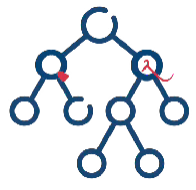
\includegraphics[height=0.9cm]{msca_logo.png}}%
  \end{center}
  \vspace{0.45cm}
  \begin{center}
    \begin{minipage}{0.1\textwidth}\centering
      \href{https://quantlet.com}{
\includegraphics[height=0.9cm]{ql_logo.png}}\end{minipage}%
    \begin{minipage}{0.78\textwidth}\centering
      {\Large\bfseries\usebeamercolor[fg]{title}\inserttitle}\par\vspace{0.25cm}
      {\large\usebeamercolor[fg]{title}\insertsubtitle}\end{minipage}%
    \begin{minipage}{0.1\textwidth}\centering
      \href{https://quantinar.com}{
\includegraphics[height=0.9cm]{qr_logo.png}}\end{minipage}
  \end{center}
  \vfill
  \hspace{0.4cm}{\bfseries\insertauthor}\par\vspace{0.12cm}
  \hspace{0.4cm}\begin{minipage}[t]{0.92\textwidth}\raggedright\footnotesize\insertinstitute\end{minipage}
  \par\vspace{0.4cm}}

% ---------------------------------------------------------------- lecture metadata
\newcommand{\nnshort}{}
\newcommand{\nnnb}{notebooks}
\newcommand{\nnrepo}{https://github.com/danpele/NEURAL_BIZ/tree/main}
% language-dependent labels (English default; \nnromanian switches to Romanian, call it before \nnlecture)
\newcommand{\txtcourse}{Neural Networks and Deep Learning}
\newcommand{\txtlecture}{Lecture}
\newcommand{\txtoutline}{Outline}
\newcommand{\txtintuition}{In one sentence:}
\newcommand{\txtjob}{In practice:}
\newcommand{\txttry}{Experiment yourself:}
\newcommand{\txtwhere}{where}
\newcommand{\txtsim}{SIMULATED DATA (teaching illustration)}
\newcommand{\txtnbsuffix}{}
\newcommand{\txtinstitute}{Bucharest University of Economic Studies (ASE), Department of Statistics and Econometrics\\
    Romanian Academy, Institute for Economic Forecasting (IPE)\\
    IDA Institute Digital Assets \textbullet\ AI4EFin \textbullet\ MSCA Digital Finance}
\newcommand{\nnromanian}{%
  \renewcommand{\txtcourse}{Rețele neuronale și deep learning}%
  \renewcommand{\txtlecture}{Cursul}%
  \renewcommand{\txtoutline}{Cuprins}%
  \renewcommand{\txtintuition}{Pe scurt:}%
  \renewcommand{\txtjob}{În practică:}%
  \renewcommand{\txttry}{Exercițiu practic:}%
  \renewcommand{\txtwhere}{unde}%
  \renewcommand{\txtsim}{DATE SIMULATE (doar pentru ilustrare)}%
  \renewcommand{\txtnbsuffix}{\string_ro}%
  \renewcommand{\txtinstitute}{Academia de Studii Economice din București (ASE), Departamentul de Statistică și Econometrie\\
    Academia Română, Institutul de Prognoză Economică (IPE)\\
    IDA Institute Digital Assets \textbullet\ AI4EFin \textbullet\ MSCA Digital Finance}}
\newcommand{\nnlecture}[2]{%
  \renewcommand{\nnshort}{\txtlecture\ #1}%
  \renewcommand{\nnnb}{notebooks/L#1\string_notebook\txtnbsuffix.ipynb}%
  \title[NN]{\txtcourse}%
  \subtitle{\txtlecture\ #1: #2}%
  \author{Prof.\ dr.\ Daniel Traian PELE}%
  \institute{\txtinstitute}%
  \date{}}

% ---------------------------------------------------------------- teaching blocks (one message per frame)
% \intuition{one plain sentence}  ->  formula with every symbol defined  ->  real-data example  ->  \manager{one line}
\newcommand{\intuition}[1]{\begin{itemize}\item {\color{MainBlue}\textbf{\txtintuition}}~#1\end{itemize}\vspace{0.6mm}}
\newcommand{\manager}[1]{\colorbox{Forest!10}{\parbox{\dimexpr\linewidth-2\fboxsep\relax}{\footnotesize
  \begin{itemize}\setlength{\itemsep}{0pt}\item \textbf{\color{Forest}\txtjob}~#1\end{itemize}}}}
% Experiment yourself: pointer to the matching notebook section
\newcommand{\tryit}[1]{{\scriptsize\href{\nnrepo/\nnnb}{%
  \raisebox{-0.15em}{
\includegraphics[height=0.85em]{ql_logo.png}}\,\textbf{\txttry}~\color{MainBlue}#1}}}
% bottom row: manager line (left) + experiment pointer (right), pinned to the bottom of the frame
\newcommand{\bottomrow}[2]{\par\vfill\noindent\begin{minipage}[b]{0.72\linewidth}#1\end{minipage}\hfill
  \begin{minipage}[b]{0.26\linewidth}\raggedleft #2\end{minipage}\par\vspace{0.5mm}}
\newcommand{\where}[1]{{\footnotesize\textbf{\txtwhere}~#1\par}}

% ---------------------------------------------------------------- helpers
% chart source line under a figure: \chartsource{Source ...; period ...}
\newcommand{\chartsource}[1]{\par\vspace{1pt}{\scriptsize\color{FooterGray}#1\par}}
% link to code: \quantlet{label}{path inside the repo}
\newcommand{\quantlet}[2]{\par\vspace{1pt}\hfill\href{\nnrepo/#2}{%
  \raisebox{-0.15em}{
\includegraphics[height=0.75em]{ql_logo.png}}\textcolor{MainBlue}{\scriptsize\ #1}}}
% inline Quantlet link for the bottom-right corner of a frame: \qlink{label}{path inside the repo}
\newcommand{\qlink}[2]{{\scriptsize\href{\nnrepo/#2}{\raisebox{-0.15em}{
\includegraphics[height=0.85em]{ql_logo.png}}\,\textcolor{MainBlue}{#1}}}}
\newcommand{\simlabel}{\colorbox{Crimson!12}{\scriptsize\bfseries\color{Crimson}\txtsim}}
\newcommand{\E}{\mathbb{E}}
\newcommand{\Var}{\operatorname{Var}}
\newcommand{\Cov}{\operatorname{Cov}}
\newcommand{\Corr}{\operatorname{Corr}}
\newcommand{\asinh}{\operatorname{asinh}}
\newcommand{\iid}{\overset{\text{i.i.d.}}{\sim}}
\newcommand{\EUR}{EUR}
% deep-learning notation (Bishop & Bishop, 2024): vectors bold lower case, matrices bold upper case
\newcommand{\R}{\mathbb{R}}
\newcommand{\vx}{\mathbf{x}}
\newcommand{\vy}{\mathbf{y}}
\newcommand{\vz}{\mathbf{z}}
\newcommand{\vh}{\mathbf{h}}
\newcommand{\vw}{\mathbf{w}}
\newcommand{\vb}{\mathbf{b}}
\newcommand{\mW}{\mathbf{W}}
\newcommand{\mX}{\mathbf{X}}
\newcommand{\btheta}{\boldsymbol{\theta}}
\newcommand{\loss}{\mathcal{L}}
\newcommand{\dataset}{\mathcal{D}}
\DeclareMathOperator*{\argmin}{arg\,min}
\DeclareMathOperator*{\argmax}{arg\,max}
\DeclareMathOperator{\softmax}{softmax}
\DeclareMathOperator{\ReLU}{ReLU}
\DeclareMathOperator{\sigm}{\sigma}

%   \nnlecture{k}{Lecture title}
% Logos live in lectures/common/logos/, charts in lectures/Lk/charts/.
% Do NOT add \hfuzz / \vfuzz / \hbadness here: overfull boxes must be fixed, not hidden.
% =============================================================================

\usetheme{default}
\setbeamersize{text margin left=7mm, text margin right=7mm}

% ---------------------------------------------------------------- packages
\usepackage[utf8]{inputenc}
\usepackage[T1]{fontenc}
\usepackage{lmodern}
\usepackage{amsmath, amssymb}
\usepackage{mathtools}
\usepackage{bm}
\usepackage{tikz}
\usetikzlibrary{arrows.meta, positioning, calc, shapes.misc}
\usepackage{booktabs}
\usepackage{array}
\usepackage{graphicx}
\usepackage{colortbl}
\usepackage{xcolor}
\usepackage{multicol}
\hypersetup{colorlinks=true, linkcolor=MainBlue, urlcolor=MainBlue, citecolor=MainBlue}
\graphicspath{{../common/logos/}}   % charts are included with their language folder: charts/en/, charts/ro/

% ---------------------------------------------------------------- colours
\definecolor{MainBlue}{RGB}{26, 58, 110}
\definecolor{IDAred}{RGB}{205, 0, 0}
\definecolor{DarkGray}{RGB}{51, 51, 51}
\definecolor{FooterGray}{RGB}{100, 100, 100}
\definecolor{BlockGray}{RGB}{236, 238, 242}
\definecolor{KeynoteGray}{RGB}{218, 218, 218}
\definecolor{Crimson}{RGB}{190, 40, 50}
\definecolor{Forest}{RGB}{30, 110, 50}
\definecolor{Bitter}{RGB}{214, 150, 20}
% chart palette (same hex values and order as lectures/common/nn_plot.py SERIES)
\definecolor{Ser1}{HTML}{2A78D6}
\definecolor{Ser2}{HTML}{EB6834}
\definecolor{Ser3}{HTML}{1BAF7A}
\definecolor{Ser4}{HTML}{EDA100}
\definecolor{Ser5}{HTML}{E87BA4}
\definecolor{Ser6}{HTML}{008300}
\definecolor{Ser7}{HTML}{6250D6}
\definecolor{Ser8}{HTML}{E34948}

\setbeamertemplate{background}{%
  \begin{tikzpicture}[remember picture, overlay]
    \shade[shading=axis, shading angle=315, top color=white, bottom color=KeynoteGray]
      (current page.south west) rectangle (current page.north east);
  \end{tikzpicture}}
\setbeamercolor{background canvas}{bg=}
\setbeamercolor{structure}{fg=MainBlue}
\setbeamercolor{normal text}{fg=DarkGray}
\setbeamercolor{title}{fg=IDAred}
\setbeamercolor{frametitle}{fg=IDAred, bg=}
\setbeamercolor{block title}{bg=MainBlue, fg=white}
\setbeamercolor{block body}{bg=BlockGray, fg=DarkGray}
\setbeamercolor{block title alerted}{bg=Crimson, fg=white}
\setbeamercolor{block body alerted}{bg=Crimson!7, fg=DarkGray}
\setbeamercolor{block title example}{bg=Forest, fg=white}
\setbeamercolor{block body example}{bg=Forest!7, fg=DarkGray}
\setbeamercolor{item}{fg=MainBlue}
\setbeamerfont{frametitle}{size=\large, series=\bfseries}
\setbeamerfont{block title}{size=\small, series=\bfseries}
\setbeamertemplate{blocks}[rounded][shadow=false]
\setbeamertemplate{itemize item}{\color{MainBlue}$\boxdot$}
\setbeamertemplate{itemize subitem}{\color{MainBlue}\scriptsize$\blacktriangleright$}
% compact two-level lists: level 1 = main point, level 2 = details (no text outside bullets)
\setbeamerfont{itemize/enumerate subbody}{size=\footnotesize}
\setlength{\leftmargini}{1.1em}
\setlength{\leftmarginii}{1.1em}
\setbeamertemplate{itemize/enumerate body begin}{\setlength{\topsep}{0pt}\setlength{\partopsep}{0pt}\setlength{\parskip}{0pt}}
\setbeamertemplate{itemize/enumerate subbody begin}{\setlength{\topsep}{0pt}\setlength{\partopsep}{0pt}\setlength{\itemsep}{0pt}\vspace{-0.4ex}}

\setbeamertemplate{enumerate item}{\color{MainBlue}\insertenumlabel.}
\setlength{\leftmargini}{1.3em}
\setlength{\leftmarginii}{1.2em}
\setbeamertemplate{navigation symbols}{}
\setbeamertemplate{section in toc}{\color{MainBlue}$\blacktriangleright$~\inserttocsection}
\setbeamertemplate{caption}{\raggedright\insertcaption\par}
% frame subtitle = precise citation line under the claim title (Weron style)
\setbeamerfont{framesubtitle}{size=\footnotesize}
\setbeamercolor{framesubtitle}{fg=FooterGray}
% outline that reappears at every section with the current section highlighted
\setbeamertemplate{section in toc shaded}[default][35]
\setbeamertemplate{subsection in toc shaded}[default][35]
\setbeamertemplate{subsection in toc}{\leavevmode\leftskip=2.2em\color{DarkGray}\small\inserttocsubsection\par}
\AtBeginSection[]{{\begin{frame}{\txtoutline}\vspace{2mm}\small
  \tableofcontents[currentsection,hideothersubsections]\end{frame}}}

% ---------------------------------------------------------------- head and foot
\setbeamertemplate{headline}{%
  \vskip10pt%
  \hbox to \paperwidth{\hskip0.5cm%
    {\small\color{FooterGray}\renewcommand{\hyperlink}[2]{##2}\insertsectionhead}%
    \hfill\textcolor{FooterGray}{\small\insertframenumber}\hskip0.5cm}%
  \vskip4pt{\color{FooterGray}\hrule height 0.4pt}}
% footer as in the other courses (MFM, SFM): course name on the left, small sparkline on the right
\setbeamertemplate{footline}{%
  {\color{FooterGray}\hrule height 0.4pt}\vskip4pt%
  \hbox to \paperwidth{\hskip0.5cm%
    \textcolor{FooterGray}{\small\txtcourse}%
    \hfill\raisebox{-0.1em}{\begin{tikzpicture}[x=0.08em, y=0.08em, line width=0.4pt]
      \draw[FooterGray] (0,3) -- (1,4) -- (2,3.5) -- (3,5) -- (4,4) -- (5,6) -- (6,5.5) -- (7,4) -- (8,5) -- (9,7) -- (10,6) -- (11,5) -- (12,6.5) -- (13,8) -- (14,7) -- (15,6) -- (16,7.5) -- (17,9) -- (18,8) -- (19,7) -- (20,8.5) -- (21,10) -- (22,9) -- (23,8) -- (24,9.5);
    \end{tikzpicture}}\hskip0.5cm}%
  \vskip6pt}

% ---------------------------------------------------------------- title page
\defbeamertemplate*{title page}{nn}[1][]{%
  \vspace{0.15cm}
  \begin{center}
    \href{https://www.ase.ro}{
\includegraphics[height=0.9cm]{ase_logo.png}}\hspace{0.3cm}%
    \href{https://ipe.ro/new}{
\includegraphics[height=0.9cm]{acad_logo.png}}\hspace{0.3cm}%
    \href{https://theida.net}{
\includegraphics[height=0.9cm]{ida_logo.png}}\hspace{0.3cm}%
    \href{https://blockchain-research-center.com}{
\includegraphics[height=0.9cm]{brc_logo.png}}\hspace{0.3cm}%
    \href{https://www.ai4efin.ase.ro}{
\includegraphics[height=0.9cm]{ai4efin_logo.png}}\hspace{0.3cm}%
    \href{https://www.digital-finance-msca.com}{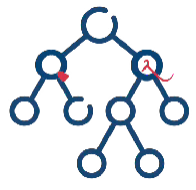
\includegraphics[height=0.9cm]{msca_logo.png}}%
  \end{center}
  \vspace{0.45cm}
  \begin{center}
    \begin{minipage}{0.1\textwidth}\centering
      \href{https://quantlet.com}{
\includegraphics[height=0.9cm]{ql_logo.png}}\end{minipage}%
    \begin{minipage}{0.78\textwidth}\centering
      {\Large\bfseries\usebeamercolor[fg]{title}\inserttitle}\par\vspace{0.25cm}
      {\large\usebeamercolor[fg]{title}\insertsubtitle}\end{minipage}%
    \begin{minipage}{0.1\textwidth}\centering
      \href{https://quantinar.com}{
\includegraphics[height=0.9cm]{qr_logo.png}}\end{minipage}
  \end{center}
  \vfill
  \hspace{0.4cm}{\bfseries\insertauthor}\par\vspace{0.12cm}
  \hspace{0.4cm}\begin{minipage}[t]{0.92\textwidth}\raggedright\footnotesize\insertinstitute\end{minipage}
  \par\vspace{0.4cm}}

% ---------------------------------------------------------------- lecture metadata
\newcommand{\nnshort}{}
\newcommand{\nnnb}{notebooks}
\newcommand{\nnrepo}{https://github.com/danpele/NEURAL_BIZ/tree/main}
% language-dependent labels (English default; \nnromanian switches to Romanian, call it before \nnlecture)
\newcommand{\txtcourse}{Neural Networks and Deep Learning}
\newcommand{\txtlecture}{Lecture}
\newcommand{\txtoutline}{Outline}
\newcommand{\txtintuition}{In one sentence:}
\newcommand{\txtjob}{In practice:}
\newcommand{\txttry}{Experiment yourself:}
\newcommand{\txtwhere}{where}
\newcommand{\txtsim}{SIMULATED DATA (teaching illustration)}
\newcommand{\txtnbsuffix}{}
\newcommand{\txtinstitute}{Bucharest University of Economic Studies (ASE), Department of Statistics and Econometrics\\
    Romanian Academy, Institute for Economic Forecasting (IPE)\\
    IDA Institute Digital Assets \textbullet\ AI4EFin \textbullet\ MSCA Digital Finance}
\newcommand{\nnromanian}{%
  \renewcommand{\txtcourse}{Rețele neuronale și deep learning}%
  \renewcommand{\txtlecture}{Cursul}%
  \renewcommand{\txtoutline}{Cuprins}%
  \renewcommand{\txtintuition}{Pe scurt:}%
  \renewcommand{\txtjob}{În practică:}%
  \renewcommand{\txttry}{Exercițiu practic:}%
  \renewcommand{\txtwhere}{unde}%
  \renewcommand{\txtsim}{DATE SIMULATE (doar pentru ilustrare)}%
  \renewcommand{\txtnbsuffix}{\string_ro}%
  \renewcommand{\txtinstitute}{Academia de Studii Economice din București (ASE), Departamentul de Statistică și Econometrie\\
    Academia Română, Institutul de Prognoză Economică (IPE)\\
    IDA Institute Digital Assets \textbullet\ AI4EFin \textbullet\ MSCA Digital Finance}}
\newcommand{\nnlecture}[2]{%
  \renewcommand{\nnshort}{\txtlecture\ #1}%
  \renewcommand{\nnnb}{notebooks/L#1\string_notebook\txtnbsuffix.ipynb}%
  \title[NN]{\txtcourse}%
  \subtitle{\txtlecture\ #1: #2}%
  \author{Prof.\ dr.\ Daniel Traian PELE}%
  \institute{\txtinstitute}%
  \date{}}

% ---------------------------------------------------------------- teaching blocks (one message per frame)
% \intuition{one plain sentence}  ->  formula with every symbol defined  ->  real-data example  ->  \manager{one line}
\newcommand{\intuition}[1]{\begin{itemize}\item {\color{MainBlue}\textbf{\txtintuition}}~#1\end{itemize}\vspace{0.6mm}}
\newcommand{\manager}[1]{\colorbox{Forest!10}{\parbox{\dimexpr\linewidth-2\fboxsep\relax}{\footnotesize
  \begin{itemize}\setlength{\itemsep}{0pt}\item \textbf{\color{Forest}\txtjob}~#1\end{itemize}}}}
% Experiment yourself: pointer to the matching notebook section
\newcommand{\tryit}[1]{{\scriptsize\href{\nnrepo/\nnnb}{%
  \raisebox{-0.15em}{
\includegraphics[height=0.85em]{ql_logo.png}}\,\textbf{\txttry}~\color{MainBlue}#1}}}
% bottom row: manager line (left) + experiment pointer (right), pinned to the bottom of the frame
\newcommand{\bottomrow}[2]{\par\vfill\noindent\begin{minipage}[b]{0.72\linewidth}#1\end{minipage}\hfill
  \begin{minipage}[b]{0.26\linewidth}\raggedleft #2\end{minipage}\par\vspace{0.5mm}}
\newcommand{\where}[1]{{\footnotesize\textbf{\txtwhere}~#1\par}}

% ---------------------------------------------------------------- helpers
% chart source line under a figure: \chartsource{Source ...; period ...}
\newcommand{\chartsource}[1]{\par\vspace{1pt}{\scriptsize\color{FooterGray}#1\par}}
% link to code: \quantlet{label}{path inside the repo}
\newcommand{\quantlet}[2]{\par\vspace{1pt}\hfill\href{\nnrepo/#2}{%
  \raisebox{-0.15em}{
\includegraphics[height=0.75em]{ql_logo.png}}\textcolor{MainBlue}{\scriptsize\ #1}}}
% inline Quantlet link for the bottom-right corner of a frame: \qlink{label}{path inside the repo}
\newcommand{\qlink}[2]{{\scriptsize\href{\nnrepo/#2}{\raisebox{-0.15em}{
\includegraphics[height=0.85em]{ql_logo.png}}\,\textcolor{MainBlue}{#1}}}}
\newcommand{\simlabel}{\colorbox{Crimson!12}{\scriptsize\bfseries\color{Crimson}\txtsim}}
\newcommand{\E}{\mathbb{E}}
\newcommand{\Var}{\operatorname{Var}}
\newcommand{\Cov}{\operatorname{Cov}}
\newcommand{\Corr}{\operatorname{Corr}}
\newcommand{\asinh}{\operatorname{asinh}}
\newcommand{\iid}{\overset{\text{i.i.d.}}{\sim}}
\newcommand{\EUR}{EUR}
% deep-learning notation (Bishop & Bishop, 2024): vectors bold lower case, matrices bold upper case
\newcommand{\R}{\mathbb{R}}
\newcommand{\vx}{\mathbf{x}}
\newcommand{\vy}{\mathbf{y}}
\newcommand{\vz}{\mathbf{z}}
\newcommand{\vh}{\mathbf{h}}
\newcommand{\vw}{\mathbf{w}}
\newcommand{\vb}{\mathbf{b}}
\newcommand{\mW}{\mathbf{W}}
\newcommand{\mX}{\mathbf{X}}
\newcommand{\btheta}{\boldsymbol{\theta}}
\newcommand{\loss}{\mathcal{L}}
\newcommand{\dataset}{\mathcal{D}}
\DeclareMathOperator*{\argmin}{arg\,min}
\DeclareMathOperator*{\argmax}{arg\,max}
\DeclareMathOperator{\softmax}{softmax}
\DeclareMathOperator{\ReLU}{ReLU}
\DeclareMathOperator{\sigm}{\sigma}

%   \nnlecture{k}{Lecture title}
% Logos live in lectures/common/logos/, charts in lectures/Lk/charts/.
% Do NOT add \hfuzz / \vfuzz / \hbadness here: overfull boxes must be fixed, not hidden.
% =============================================================================

\usetheme{default}
\setbeamersize{text margin left=7mm, text margin right=7mm}

% ---------------------------------------------------------------- packages
\usepackage[utf8]{inputenc}
\usepackage[T1]{fontenc}
\usepackage{lmodern}
\usepackage{amsmath, amssymb}
\usepackage{mathtools}
\usepackage{bm}
\usepackage{tikz}
\usetikzlibrary{arrows.meta, positioning, calc, shapes.misc}
\usepackage{booktabs}
\usepackage{array}
\usepackage{graphicx}
\usepackage{colortbl}
\usepackage{xcolor}
\usepackage{multicol}
\hypersetup{colorlinks=true, linkcolor=MainBlue, urlcolor=MainBlue, citecolor=MainBlue}
\graphicspath{{../common/logos/}}   % charts are included with their language folder: charts/en/, charts/ro/

% ---------------------------------------------------------------- colours
\definecolor{MainBlue}{RGB}{26, 58, 110}
\definecolor{IDAred}{RGB}{205, 0, 0}
\definecolor{DarkGray}{RGB}{51, 51, 51}
\definecolor{FooterGray}{RGB}{100, 100, 100}
\definecolor{BlockGray}{RGB}{236, 238, 242}
\definecolor{KeynoteGray}{RGB}{218, 218, 218}
\definecolor{Crimson}{RGB}{190, 40, 50}
\definecolor{Forest}{RGB}{30, 110, 50}
\definecolor{Bitter}{RGB}{214, 150, 20}
% chart palette (same hex values and order as lectures/common/nn_plot.py SERIES)
\definecolor{Ser1}{HTML}{2A78D6}
\definecolor{Ser2}{HTML}{EB6834}
\definecolor{Ser3}{HTML}{1BAF7A}
\definecolor{Ser4}{HTML}{EDA100}
\definecolor{Ser5}{HTML}{E87BA4}
\definecolor{Ser6}{HTML}{008300}
\definecolor{Ser7}{HTML}{6250D6}
\definecolor{Ser8}{HTML}{E34948}

\setbeamertemplate{background}{%
  \begin{tikzpicture}[remember picture, overlay]
    \shade[shading=axis, shading angle=315, top color=white, bottom color=KeynoteGray]
      (current page.south west) rectangle (current page.north east);
  \end{tikzpicture}}
\setbeamercolor{background canvas}{bg=}
\setbeamercolor{structure}{fg=MainBlue}
\setbeamercolor{normal text}{fg=DarkGray}
\setbeamercolor{title}{fg=IDAred}
\setbeamercolor{frametitle}{fg=IDAred, bg=}
\setbeamercolor{block title}{bg=MainBlue, fg=white}
\setbeamercolor{block body}{bg=BlockGray, fg=DarkGray}
\setbeamercolor{block title alerted}{bg=Crimson, fg=white}
\setbeamercolor{block body alerted}{bg=Crimson!7, fg=DarkGray}
\setbeamercolor{block title example}{bg=Forest, fg=white}
\setbeamercolor{block body example}{bg=Forest!7, fg=DarkGray}
\setbeamercolor{item}{fg=MainBlue}
\setbeamerfont{frametitle}{size=\large, series=\bfseries}
\setbeamerfont{block title}{size=\small, series=\bfseries}
\setbeamertemplate{blocks}[rounded][shadow=false]
\setbeamertemplate{itemize item}{\color{MainBlue}$\boxdot$}
\setbeamertemplate{itemize subitem}{\color{MainBlue}\scriptsize$\blacktriangleright$}
% compact two-level lists: level 1 = main point, level 2 = details (no text outside bullets)
\setbeamerfont{itemize/enumerate subbody}{size=\footnotesize}
\setlength{\leftmargini}{1.1em}
\setlength{\leftmarginii}{1.1em}
\setbeamertemplate{itemize/enumerate body begin}{\setlength{\topsep}{0pt}\setlength{\partopsep}{0pt}\setlength{\parskip}{0pt}}
\setbeamertemplate{itemize/enumerate subbody begin}{\setlength{\topsep}{0pt}\setlength{\partopsep}{0pt}\setlength{\itemsep}{0pt}\vspace{-0.4ex}}

\setbeamertemplate{enumerate item}{\color{MainBlue}\insertenumlabel.}
\setlength{\leftmargini}{1.3em}
\setlength{\leftmarginii}{1.2em}
\setbeamertemplate{navigation symbols}{}
\setbeamertemplate{section in toc}{\color{MainBlue}$\blacktriangleright$~\inserttocsection}
\setbeamertemplate{caption}{\raggedright\insertcaption\par}
% frame subtitle = precise citation line under the claim title (Weron style)
\setbeamerfont{framesubtitle}{size=\footnotesize}
\setbeamercolor{framesubtitle}{fg=FooterGray}
% outline that reappears at every section with the current section highlighted
\setbeamertemplate{section in toc shaded}[default][35]
\setbeamertemplate{subsection in toc shaded}[default][35]
\setbeamertemplate{subsection in toc}{\leavevmode\leftskip=2.2em\color{DarkGray}\small\inserttocsubsection\par}
\AtBeginSection[]{{\begin{frame}{\txtoutline}\vspace{2mm}\small
  \tableofcontents[currentsection,hideothersubsections]\end{frame}}}

% ---------------------------------------------------------------- head and foot
\setbeamertemplate{headline}{%
  \vskip10pt%
  \hbox to \paperwidth{\hskip0.5cm%
    {\small\color{FooterGray}\renewcommand{\hyperlink}[2]{##2}\insertsectionhead}%
    \hfill\textcolor{FooterGray}{\small\insertframenumber}\hskip0.5cm}%
  \vskip4pt{\color{FooterGray}\hrule height 0.4pt}}
% footer as in the other courses (MFM, SFM): course name on the left, small sparkline on the right
\setbeamertemplate{footline}{%
  {\color{FooterGray}\hrule height 0.4pt}\vskip4pt%
  \hbox to \paperwidth{\hskip0.5cm%
    \textcolor{FooterGray}{\small\txtcourse}%
    \hfill\raisebox{-0.1em}{\begin{tikzpicture}[x=0.08em, y=0.08em, line width=0.4pt]
      \draw[FooterGray] (0,3) -- (1,4) -- (2,3.5) -- (3,5) -- (4,4) -- (5,6) -- (6,5.5) -- (7,4) -- (8,5) -- (9,7) -- (10,6) -- (11,5) -- (12,6.5) -- (13,8) -- (14,7) -- (15,6) -- (16,7.5) -- (17,9) -- (18,8) -- (19,7) -- (20,8.5) -- (21,10) -- (22,9) -- (23,8) -- (24,9.5);
    \end{tikzpicture}}\hskip0.5cm}%
  \vskip6pt}

% ---------------------------------------------------------------- title page
\defbeamertemplate*{title page}{nn}[1][]{%
  \vspace{0.15cm}
  \begin{center}
    \href{https://www.ase.ro}{
\includegraphics[height=0.9cm]{ase_logo.png}}\hspace{0.3cm}%
    \href{https://ipe.ro/new}{
\includegraphics[height=0.9cm]{acad_logo.png}}\hspace{0.3cm}%
    \href{https://theida.net}{
\includegraphics[height=0.9cm]{ida_logo.png}}\hspace{0.3cm}%
    \href{https://blockchain-research-center.com}{
\includegraphics[height=0.9cm]{brc_logo.png}}\hspace{0.3cm}%
    \href{https://www.ai4efin.ase.ro}{
\includegraphics[height=0.9cm]{ai4efin_logo.png}}\hspace{0.3cm}%
    \href{https://www.digital-finance-msca.com}{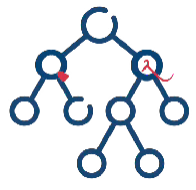
\includegraphics[height=0.9cm]{msca_logo.png}}%
  \end{center}
  \vspace{0.45cm}
  \begin{center}
    \begin{minipage}{0.1\textwidth}\centering
      \href{https://quantlet.com}{
\includegraphics[height=0.9cm]{ql_logo.png}}\end{minipage}%
    \begin{minipage}{0.78\textwidth}\centering
      {\Large\bfseries\usebeamercolor[fg]{title}\inserttitle}\par\vspace{0.25cm}
      {\large\usebeamercolor[fg]{title}\insertsubtitle}\end{minipage}%
    \begin{minipage}{0.1\textwidth}\centering
      \href{https://quantinar.com}{
\includegraphics[height=0.9cm]{qr_logo.png}}\end{minipage}
  \end{center}
  \vfill
  \hspace{0.4cm}{\bfseries\insertauthor}\par\vspace{0.12cm}
  \hspace{0.4cm}\begin{minipage}[t]{0.92\textwidth}\raggedright\footnotesize\insertinstitute\end{minipage}
  \par\vspace{0.4cm}}

% ---------------------------------------------------------------- lecture metadata
\newcommand{\nnshort}{}
\newcommand{\nnnb}{notebooks}
\newcommand{\nnrepo}{https://github.com/danpele/NEURAL_BIZ/tree/main}
% language-dependent labels (English default; \nnromanian switches to Romanian, call it before \nnlecture)
\newcommand{\txtcourse}{Neural Networks and Deep Learning}
\newcommand{\txtlecture}{Lecture}
\newcommand{\txtoutline}{Outline}
\newcommand{\txtintuition}{In one sentence:}
\newcommand{\txtjob}{In practice:}
\newcommand{\txttry}{Experiment yourself:}
\newcommand{\txtwhere}{where}
\newcommand{\txtsim}{SIMULATED DATA (teaching illustration)}
\newcommand{\txtnbsuffix}{}
\newcommand{\txtinstitute}{Bucharest University of Economic Studies (ASE), Department of Statistics and Econometrics\\
    Romanian Academy, Institute for Economic Forecasting (IPE)\\
    IDA Institute Digital Assets \textbullet\ AI4EFin \textbullet\ MSCA Digital Finance}
\newcommand{\nnromanian}{%
  \renewcommand{\txtcourse}{Rețele neuronale și deep learning}%
  \renewcommand{\txtlecture}{Cursul}%
  \renewcommand{\txtoutline}{Cuprins}%
  \renewcommand{\txtintuition}{Pe scurt:}%
  \renewcommand{\txtjob}{În practică:}%
  \renewcommand{\txttry}{Exercițiu practic:}%
  \renewcommand{\txtwhere}{unde}%
  \renewcommand{\txtsim}{DATE SIMULATE (doar pentru ilustrare)}%
  \renewcommand{\txtnbsuffix}{\string_ro}%
  \renewcommand{\txtinstitute}{Academia de Studii Economice din București (ASE), Departamentul de Statistică și Econometrie\\
    Academia Română, Institutul de Prognoză Economică (IPE)\\
    IDA Institute Digital Assets \textbullet\ AI4EFin \textbullet\ MSCA Digital Finance}}
\newcommand{\nnlecture}[2]{%
  \renewcommand{\nnshort}{\txtlecture\ #1}%
  \renewcommand{\nnnb}{notebooks/L#1\string_notebook\txtnbsuffix.ipynb}%
  \title[NN]{\txtcourse}%
  \subtitle{\txtlecture\ #1: #2}%
  \author{Prof.\ dr.\ Daniel Traian PELE}%
  \institute{\txtinstitute}%
  \date{}}

% ---------------------------------------------------------------- teaching blocks (one message per frame)
% \intuition{one plain sentence}  ->  formula with every symbol defined  ->  real-data example  ->  \manager{one line}
\newcommand{\intuition}[1]{\begin{itemize}\item {\color{MainBlue}\textbf{\txtintuition}}~#1\end{itemize}\vspace{0.6mm}}
\newcommand{\manager}[1]{\colorbox{Forest!10}{\parbox{\dimexpr\linewidth-2\fboxsep\relax}{\footnotesize
  \begin{itemize}\setlength{\itemsep}{0pt}\item \textbf{\color{Forest}\txtjob}~#1\end{itemize}}}}
% Experiment yourself: pointer to the matching notebook section
\newcommand{\tryit}[1]{{\scriptsize\href{\nnrepo/\nnnb}{%
  \raisebox{-0.15em}{
\includegraphics[height=0.85em]{ql_logo.png}}\,\textbf{\txttry}~\color{MainBlue}#1}}}
% bottom row: manager line (left) + experiment pointer (right), pinned to the bottom of the frame
\newcommand{\bottomrow}[2]{\par\vfill\noindent\begin{minipage}[b]{0.72\linewidth}#1\end{minipage}\hfill
  \begin{minipage}[b]{0.26\linewidth}\raggedleft #2\end{minipage}\par\vspace{0.5mm}}
\newcommand{\where}[1]{{\footnotesize\textbf{\txtwhere}~#1\par}}

% ---------------------------------------------------------------- helpers
% chart source line under a figure: \chartsource{Source ...; period ...}
\newcommand{\chartsource}[1]{\par\vspace{1pt}{\scriptsize\color{FooterGray}#1\par}}
% link to code: \quantlet{label}{path inside the repo}
\newcommand{\quantlet}[2]{\par\vspace{1pt}\hfill\href{\nnrepo/#2}{%
  \raisebox{-0.15em}{
\includegraphics[height=0.75em]{ql_logo.png}}\textcolor{MainBlue}{\scriptsize\ #1}}}
% inline Quantlet link for the bottom-right corner of a frame: \qlink{label}{path inside the repo}
\newcommand{\qlink}[2]{{\scriptsize\href{\nnrepo/#2}{\raisebox{-0.15em}{
\includegraphics[height=0.85em]{ql_logo.png}}\,\textcolor{MainBlue}{#1}}}}
\newcommand{\simlabel}{\colorbox{Crimson!12}{\scriptsize\bfseries\color{Crimson}\txtsim}}
\newcommand{\E}{\mathbb{E}}
\newcommand{\Var}{\operatorname{Var}}
\newcommand{\Cov}{\operatorname{Cov}}
\newcommand{\Corr}{\operatorname{Corr}}
\newcommand{\asinh}{\operatorname{asinh}}
\newcommand{\iid}{\overset{\text{i.i.d.}}{\sim}}
\newcommand{\EUR}{EUR}
% deep-learning notation (Bishop & Bishop, 2024): vectors bold lower case, matrices bold upper case
\newcommand{\R}{\mathbb{R}}
\newcommand{\vx}{\mathbf{x}}
\newcommand{\vy}{\mathbf{y}}
\newcommand{\vz}{\mathbf{z}}
\newcommand{\vh}{\mathbf{h}}
\newcommand{\vw}{\mathbf{w}}
\newcommand{\vb}{\mathbf{b}}
\newcommand{\mW}{\mathbf{W}}
\newcommand{\mX}{\mathbf{X}}
\newcommand{\btheta}{\boldsymbol{\theta}}
\newcommand{\loss}{\mathcal{L}}
\newcommand{\dataset}{\mathcal{D}}
\DeclareMathOperator*{\argmin}{arg\,min}
\DeclareMathOperator*{\argmax}{arg\,max}
\DeclareMathOperator{\softmax}{softmax}
\DeclareMathOperator{\ReLU}{ReLU}
\DeclareMathOperator{\sigm}{\sigma}

\nnlecture{10}{Reinforcement learning: trading, hedging and battery dispatch}
\begin{document}
{\setbeamertemplate{headline}{}\setbeamertemplate{footline}{}
\begin{frame}\titlepage\end{frame}}
% END-FRONT-MATTER

\begin{frame}{Learning objectives}
\small
\begin{itemize}\setlength{\itemsep}{4pt}
  \item Write a business decision as a Markov decision process (MDP): state, action, reward, transition and discount.
  \item Solve a small MDP exactly with the Bellman equation and dynamic programming (DP), and read the value function.
  \item Train value-based agents (tabular Q-learning, a deep Q-network (DQN)) and a policy-gradient agent (proximal policy optimisation (PPO)) on real prices, with several seeds and an honest benchmark.
  \item Hedge an option with a neural policy that minimises the expected shortfall (ES) of the loss, and compare it with the Black-Scholes delta.
  \item Judge when reinforcement learning (RL) adds value in business and when a simple rule is enough.
\end{itemize}
\end{frame}

% BEGIN-ABBR

\begin{frame}{Abbreviations}
\small
\vspace{-1mm}\begin{columns}[T,onlytextwidth]
\begin{column}{0.49\textwidth}{\scriptsize\renewcommand{\arraystretch}{0.96}\begin{tabular}{@{}>{\bfseries}l@{\ \ }p{0.74\linewidth}@{}}A2C & advantage actor-critic\\
AI & artificial intelligence\\
ASE & Bucharest University of Economic Studies\\
ATM & at the money (strike = current price)\\
BG & Bulgaria (bidding zone)\\
CET & Central European Time\\
CPU & central processing unit\\
DE-LU & Germany-Luxembourg bidding zone\\
DM & Diebold-Mariano test\\
DP & dynamic programming\\
DQN & deep Q-network\\
ENTSO-E & European Network of Transmission System Operators for Electricity\\
ES & expected shortfall\\
EU & European Union\\
EUR & euro\\
GAE & generalised advantage estimation\\
HU & Hungary (bidding zone)\\\end{tabular}}\end{column}
\begin{column}{0.49\textwidth}{\scriptsize\renewcommand{\arraystretch}{0.96}\begin{tabular}{@{}>{\bfseries}l@{\ \ }p{0.74\linewidth}@{}}IPE & Institute for Economic Forecasting, Romanian Academy\\
ISE & Fraunhofer Institute for Solar Energy Systems\\
KL & Kullback-Leibler divergence\\
MDP & Markov decision process\\
MLP & multilayer perceptron\\
MW & megawatt\\
MWh & megawatt-hour\\
PPO & proximal policy optimisation\\
ReLU & rectified linear unit\\
RL & reinforcement learning\\
RO & Romania (bidding zone)\\
SSRN & Social Science Research Network\\
TD & temporal difference\\
TRPO & trust region policy optimisation\\
USD & US dollar\\
VaR & value at risk\\
VIX & Cboe Volatility Index (30-day implied volatility of the S\&P 500)\\\end{tabular}}\end{column}
\end{columns}
\end{frame}

% END-ABBR

\begin{frame}{Real data in this lecture}
\footnotesize
\begin{itemize}\setlength{\itemsep}{2pt}
  \item Three problems, three real datasets
    \begin{itemize}\setlength{\itemsep}{0pt}
      \item Every number on the slides is computed by analysis\_L10.py and stored in L10\_numbers.json.
    \end{itemize}
\end{itemize}\vspace{1mm}{\footnotesize\renewcommand{\arraystretch}{1.05}\setlength{\tabcolsep}{4pt}
\begin{tabular}{@{}p{0.2\textwidth}p{0.4\textwidth}p{0.33\textwidth}@{}}\toprule
Problem & Data and source & Split (time order) \\ \midrule
Battery dispatch & Hourly day-ahead prices, Romania (RO), Hungary (HU), Germany-Luxembourg (DE-LU), Bulgaria (BG); energy-charts.info of the Fraunhofer Institute for Solar Energy Systems (ISE), from data of the European Network of Transmission System Operators for Electricity (ENTSO-E) & train 2019--2023, validation 2024, test 1 Jan 2025 -- 24 Oct 2026 \\
Trading & S\&P 500 daily closes and the Cboe Volatility Index (VIX); Yahoo Finance & train 2005--2016, validation 2017--2019, test 2020 -- 29 Oct 2026 \\
Option hedging & 21-day S\&P 500 paths, VIX as implied volatility & paths starting 2005--2016 / 2017--2019 / 2020 -- 1 Oct 2026 \\
\bottomrule\end{tabular}}\begin{itemize}\setlength{\itemsep}{1pt}
  \item Data cut at 31 Oct 2026, the last complete month
    \begin{itemize}\setlength{\itemsep}{0pt}
      \item Seeds 20261108 to 20261108+4
      \item Training on an Apple M5 Max central processing unit (CPU), trained results cached.
    \end{itemize}
\end{itemize}
\end{frame}


\section{Sequential decisions in business}

\begin{frame}{Reinforcement learning: learning what to do, not what will happen}
\footnotesize
\intuition{supervised learning predicts a label; RL chooses actions whose consequences arrive later and depend on what it did before.}
\begin{columns}[T,onlytextwidth]
\begin{column}{0.53\textwidth}
\begin{itemize}\setlength{\itemsep}{2pt}
  \item \textbf{Supervised}
    \begin{itemize}\setlength{\itemsep}{0pt}
      \item Data $(\vx_i, y_i)$, loss $\loss(\hat y_i, y_i)$ known for each example
      \item The prediction does not change the next example
    \end{itemize}
  \item \textbf{Reinforcement}
    \begin{itemize}\setlength{\itemsep}{0pt}
      \item The agent sees a state $s_t$, acts $a_t$, receives a reward $r_{t+1}$
      \item The action changes the next state (a full battery cannot charge)
      \item No teacher gives the right action: only a delayed, noisy reward
    \end{itemize}
\end{itemize}
\end{column}
\begin{column}{0.44\textwidth}
\begin{itemize}\setlength{\itemsep}{2pt}
  \item \textbf{Business decisions of this kind}
    \begin{itemize}\setlength{\itemsep}{0pt}
      \item Storage: when to charge and discharge
      \item Trading: when to be in or out of the market
      \item Hedging: how much of the underlying to hold each day
      \item Inventory, pricing, credit limits
    \end{itemize}
\end{itemize}
\end{column}
\end{columns}
\par\vfill\manager{use RL only when today's action changes tomorrow's options.}\par\vspace{0.5mm}
\par\vfill\noindent{\scriptsize\color{FooterGray}(Sutton \& Barto, 2018, ch.\ 1)}\par\vspace{0.5mm}
\end{frame}

\begin{frame}{The agent-environment loop}
\small
\intuition{the agent acts, the environment answers with a reward and a new state; learning means improving the policy from these answers.}
\begin{center}\begin{tikzpicture}[node distance=2.6cm, every node/.style={font=\footnotesize}]
\node[draw, rounded corners, fill=Ser2!20, minimum width=2.6cm, minimum height=0.6cm] (ag) {Agent: policy $\pi_{\btheta}(a\mid s)$};
\node[draw, rounded corners, fill=Ser1!15, minimum width=2.6cm, minimum height=0.6cm, right=4.2cm of ag] (env) {Environment: market, battery};
\draw[-{Latex}, thick] (ag.north) to[bend left=12] node[above]{action $a_t$} (env.north);
\draw[-{Latex}, thick] (env.south) to[bend left=12] node[below]{reward $r_{t+1}$, new state $s_{t+1}$} (ag.south);
\end{tikzpicture}\end{center}\begin{itemize}\setlength{\itemsep}{0pt}
  \item \textbf{Episode}: a delivery day, a 126-day trading window, a 21-day option life.
  \item \textbf{Model-free}: the agent learns from sampled transitions $(s_t,a_t,r_{t+1},s_{t+1})$, never from the transition law.
  \item \textbf{Offline here}: all three agents learn from historical data.
\end{itemize}
\par\vfill\manager{write down state, action and reward before training anything.}\par\vspace{0.5mm}
\par\vfill\noindent{\scriptsize\color{FooterGray}(Sutton \& Barto, 2018, ch.\ 3)}\par\vspace{0.5mm}
\end{frame}

\begin{frame}{Three business problems, one framework}
\footnotesize
{\footnotesize\renewcommand{\arraystretch}{1.05}\setlength{\tabcolsep}{4pt}
\begin{tabular}{@{}p{0.14\textwidth}p{0.27\textwidth}p{0.2\textwidth}p{0.33\textwidth}@{}}\toprule
Problem & State $s_t$ & Action $a_t$ & Reward $r_{t+1}$ \\ \midrule
Battery & hour, stored energy, yesterday's prices & charge / idle / discharge & cash flow of the hour (EUR) \\
Trading & past returns, volatility, VIX, trend, current position & flat / long & position $\times$ next return $-$ cost \\
Hedging & index level, time to maturity, VIX, previous hedge & hedge ratio $\delta_t\in[0,1]$ & terminal profit and loss, judged by its ES \\
\bottomrule\end{tabular}}\vspace{1mm}\begin{itemize}\setlength{\itemsep}{2pt}
  \item Same mathematics: maximise expected discounted reward
    \begin{itemize}\setlength{\itemsep}{0pt}
      \item Different information and different risk attitudes.
    \end{itemize}
  \item Benchmarks are rules a manager already uses: yesterday's plan, buy-and-hold, the 200-day moving average, Black-Scholes delta.
\end{itemize}
\par\vfill\manager{an RL agent is worth deploying only if it beats the rule the desk already uses, after costs and over several seeds.}\par\vspace{0.5mm}
\par\vfill\noindent{\scriptsize\color{FooterGray}(own computation)}\par\vspace{0.5mm}
\end{frame}

\begin{frame}{Batteries earn the daily price spread, and the spread has grown}
\small
\intuition{a battery buys in the cheapest hours and sells in the dearest; its income scales with the daily max-min spread.}
\begin{center}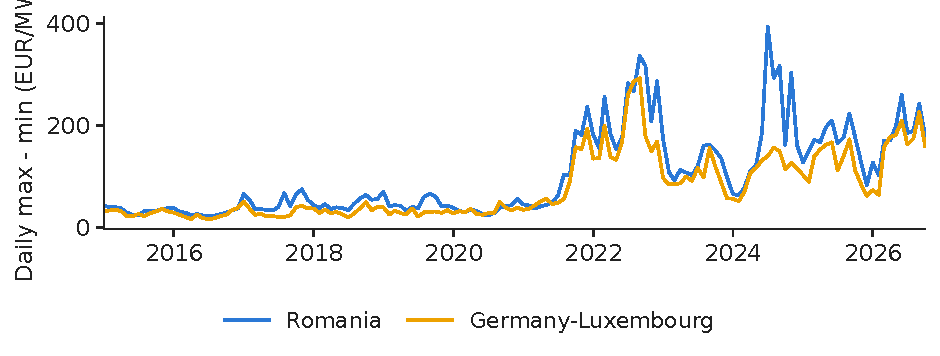
\includegraphics[width=\textwidth,height=0.342\textheight,keepaspectratio]{charts/en/spread_monthly.pdf}\end{center}\vspace{-3mm}
\chartsource{Source: energy-charts.info (Fraunhofer ISE), from exchange and ENTSO-E data. Data: 2 Jan 2015 to 31 Oct 2026, monthly mean of the daily spread.}
\vspace{0.5mm}
\begin{itemize}\setlength{\itemsep}{0pt}
  \item Romania: mean daily spread 47.9 EUR/MWh in 2019, 164.3 in 2025, 182.8 in 2026 so far.
  \item Peak month Jul 2024: 394.4 EUR/MWh
    \begin{itemize}\setlength{\itemsep}{0pt}
      \item Solar output now pushes midday prices down.
    \end{itemize}
\end{itemize}
\par\vfill\manager{the business case of a battery is a bet on future spreads, not on the price level.}\par\vspace{0.5mm}
\par\vfill\noindent{\scriptsize\color{FooterGray}(own computation)}\hfill\qlink{NN\_L10\_spread\_monthly}{Quantlets/L10/NN_L10_spread_monthly}\par\vspace{0.5mm}
\end{frame}


\section{Markov decision processes and the Bellman equation}

\begin{frame}{A Markov decision process has five ingredients}
\footnotesize
\intuition{the future depends on the past only through the current state and action.}
\begin{columns}[T,onlytextwidth]
\begin{column}{0.52\textwidth}
\[ \mathcal{M}=(\mathcal{S},\mathcal{A},P,R,\gamma) \]\[ P(s'\mid s,a)=\Pr(s_{t+1}=s'\mid s_t=s,a_t=a) \]\[ G_t=\sum_{k=0}^{T-t-1}\gamma^{k}r_{t+k+1},\quad \pi^{*}=\argmax_{\pi}\E_{\pi}[G_0] \]{\footnotesize\begin{itemize}\setlength{\itemsep}{0pt}
  \item \textbf{\txtwhere}
    \begin{itemize}\setlength{\itemsep}{0pt}
      \item $\mathcal{S},\mathcal{A}$ = states and actions, $P$ = transition law, $R(s,a)=\E[r_{t+1}\mid s,a]$
      \item $\gamma\in[0,1]$ = discount factor, $G_t$ = return, $\pi(a\mid s)$ = policy.
    \end{itemize}
\end{itemize}\par}
\end{column}
\begin{column}{0.45\textwidth}
\begin{itemize}\setlength{\itemsep}{3pt}
  \item \textbf{Markov property}: the state must contain everything relevant
    \begin{itemize}\setlength{\itemsep}{0pt}
      \item For the battery: hour and stored energy
      \item For trading: the current position, because it determines the cost of the next trade.
    \end{itemize}
  \item \textbf{Discounting}: $\gamma=1$ for one-day battery episodes (24 steps), $\gamma=0.99$ for trading.
  \item \textbf{Finite horizon}: the battery starts each day empty and its value at midnight is zero.
\end{itemize}
\end{column}
\end{columns}
\par\vfill\manager{a missing state variable, such as the current position, makes the agent erratic.}\par\vspace{0.5mm}
\par\vfill\noindent{\scriptsize\color{FooterGray}(Sutton \& Barto, 2018, ch.\ 3)}\par\vspace{0.5mm}
\end{frame}

\begin{frame}{Value functions measure how good a state is}
\footnotesize
\intuition{$V$ is the expected future reward from a state; $Q$ is the same after a given first action.}
\begin{columns}[T,onlytextwidth]
\begin{column}{0.52\textwidth}
\[ V^{\pi}(s)=\E_{\pi}[G_t\mid s_t=s] \]\[ Q^{\pi}(s,a)=\E_{\pi}[G_t\mid s_t=s,a_t=a] \]\[ A^{\pi}(s,a)=Q^{\pi}(s,a)-V^{\pi}(s) \]{\footnotesize\begin{itemize}\setlength{\itemsep}{0pt}
  \item \textbf{\txtwhere}
    \begin{itemize}\setlength{\itemsep}{0pt}
      \item $A^{\pi}$ = advantage of action $a$ over the policy's average action
      \item The optimal policy is greedy in $Q^{*}$: $\pi^{*}(s)=\argmax_a Q^{*}(s,a)$.
    \end{itemize}
\end{itemize}\par}
\end{column}
\begin{column}{0.45\textwidth}
\begin{itemize}\setlength{\itemsep}{3pt}
  \item \textbf{Value-based methods} (Q-learning, DQN) estimate $Q^{*}$ and act greedily.
  \item \textbf{Policy-based methods} (REINFORCE, PPO) parameterise $\pi_{\btheta}$ directly and use $V$ only as a baseline.
  \item \textbf{Battery example}: $V_h(s)$ = the euros still to be earned today from hour $h$ with $s$ MWh stored.
\end{itemize}
\end{column}
\end{columns}
\par\vfill\manager{$V$ prices an asset (a charged battery, an open position)
    \begin{itemize}\setlength{\itemsep}{0pt}
      \item $Q$ compares decisions.
    \end{itemize}}\par\vspace{0.5mm}
\par\vfill\noindent{\scriptsize\color{FooterGray}(Sutton \& Barto, 2018, ch.\ 3--4)}\par\vspace{0.5mm}
\end{frame}

\begin{frame}{The Bellman equation turns a long problem into one-step problems}
\footnotesize
\intuition{the best value now = best immediate reward + discounted best value of where you land.}
\begin{columns}[T,onlytextwidth]
\begin{column}{0.53\textwidth}
\[ V^{*}(s)=\max_{a}\Big\{R(s,a)+\gamma\sum_{s'}P(s'\mid s,a)\,V^{*}(s')\Big\} \]\[ Q^{*}(s,a)=R(s,a)+\gamma\,\E_{s'}\big[\max_{a'}Q^{*}(s',a')\big] \]{\footnotesize\begin{itemize}\setlength{\itemsep}{0pt}
  \item \textbf{\txtwhere}
    \begin{itemize}\setlength{\itemsep}{0pt}
      \item The right-hand side is a contraction for $\gamma<1$, so value iteration $V_{k+1}=\mathcal{T}V_k$ converges to the unique fixed point $V^{*}$
      \item With a finite horizon, one backward pass is exact.
    \end{itemize}
\end{itemize}\par}
\end{column}
\begin{column}{0.44\textwidth}
\begin{itemize}\setlength{\itemsep}{3pt}
  \item \textbf{Principle of optimality} (Bellman, 1957): an optimal plan stays optimal from any intermediate state.
  \item \textbf{Curse of dimensionality}: the table has $|\mathcal{S}|\times|\mathcal{A}|$ cells
    \begin{itemize}\setlength{\itemsep}{0pt}
      \item Neural networks replace the table when the state is large.
    \end{itemize}
  \item \textbf{Model needed}: DP uses $P$ and $R$
    \begin{itemize}\setlength{\itemsep}{0pt}
      \item Q-learning and DQN replace the expectation by samples.
    \end{itemize}
\end{itemize}
\end{column}
\end{columns}
\par\vfill\manager{every RL algorithm in this lecture is an approximate way to solve this equation.}\par\vspace{0.5mm}
\par\vfill\noindent{\scriptsize\color{FooterGray}(Bellman, 1957; Sutton \& Barto, 2018, ch.\ 4)}\par\vspace{0.5mm}
\end{frame}

\begin{frame}{The battery as an MDP}
\footnotesize
\intuition{state = (hour, stored energy); action = charge, idle or discharge; reward = the cash flow of the hour.}
\begin{columns}[T,onlytextwidth]
\begin{column}{0.5\textwidth}
\[ s_{h+1}=s_h-a_h,\quad s_h\in\{0,1,2\}\ \text{MWh},\quad a_h\in\{-1,0,+1\} \]\[ r_h(a_h)=\begin{cases}\eta_d\,p_h & a_h=+1\ (sell)\\ -p_h/\eta_c & a_h=-1\ (buy)\\ 0 & a_h=0\end{cases} \]{\footnotesize\begin{itemize}\setlength{\itemsep}{0pt}
  \item \textbf{\txtwhere}
    \begin{itemize}\setlength{\itemsep}{0pt}
      \item $p_h$ = day-ahead price of hour $h$ (EUR/MWh), $\eta_c=\eta_d=\sqrt{0.85}$ (85\,\% round trip)
      \item 2 MWh, 1 MWh moved per hour, empty at 0:00.
    \end{itemize}
\end{itemize}\par}
\end{column}
\begin{column}{0.47\textwidth}
\begin{itemize}\setlength{\itemsep}{3pt}
  \item \textbf{Constraint}: no charging when full, no discharging when empty (action masking).
  \item \textbf{Data}: 4\,292 Romanian delivery days with 24 complete hours, 2 Jan 2015 -- 31 Oct 2026
    \begin{itemize}\setlength{\itemsep}{0pt}
      \item Since Oct 2025 the hour is the mean of four 15-minute prices.
    \end{itemize}
  \item \textbf{Simplifications}: price taker, no degradation cost, no grid fees, no ancillary services.
\end{itemize}
\end{column}
\end{columns}
\par\vfill\manager{the stored energy is what makes the decision sequential.}\par\vspace{0.5mm}
\par\vfill\noindent{\scriptsize\color{FooterGray}(own computation)}\hfill\tryit{notebook \S2}\par\vspace{0.5mm}
\end{frame}

\begin{frame}{Dynamic programming solves the battery day exactly}
\footnotesize
\intuition{go backwards from midnight: at each hour, keep the best action for each level of stored energy.}
\begin{columns}[T,onlytextwidth]
\begin{column}{0.53\textwidth}
\[ V_{24}(s)=0 \]\[ V_h(s)=\max_{a:\,0\le s-a\le 2}\big\{r_h(a)+V_{h+1}(s-a)\big\},\quad h=23,\dots,0 \]{\footnotesize\begin{itemize}\setlength{\itemsep}{0pt}
  \item \textbf{\txtwhere}
    \begin{itemize}\setlength{\itemsep}{0pt}
      \item $V_h(s)$ = maximal cash flow from hour $h$ to midnight with $s$ MWh stored
      \item The revenue of the day is $V_0(0)$
      \item The argmax at each $(h,s)$ is the optimal action.
    \end{itemize}
\end{itemize}\par}
\end{column}
\begin{column}{0.44\textwidth}
\begin{itemize}\setlength{\itemsep}{3pt}
  \item \textbf{Cost}: $24\times3\times3$ evaluations per day
    \begin{itemize}\setlength{\itemsep}{0pt}
      \item All 4\,292 days in milliseconds, vectorised over days.
    \end{itemize}
  \item \textbf{Perfect foresight}: DP uses the day's 24 prices before they are known, so its revenue is an \textbf{upper bound} for any real strategy.
  \item \textbf{Naive benchmark}: compute yesterday's optimal plan and apply it today.
\end{itemize}
\end{column}
\end{columns}
\par\vfill\manager{DP gives the ceiling against which every learning agent is scored (capture ratio = revenue / perfect-foresight revenue).}\par\vspace{0.5mm}
\par\vfill\noindent{\scriptsize\color{FooterGray}(Bellman, 1957)}\hfill\tryit{notebook \S2}\par\vspace{0.5mm}
\end{frame}

\begin{frame}{One real day: buy at the trough, sell at the peaks}
\small
\intuition{on the day with the largest spread of 2026, DP charges in the cheapest hours and discharges in the dearest.}
\begin{center}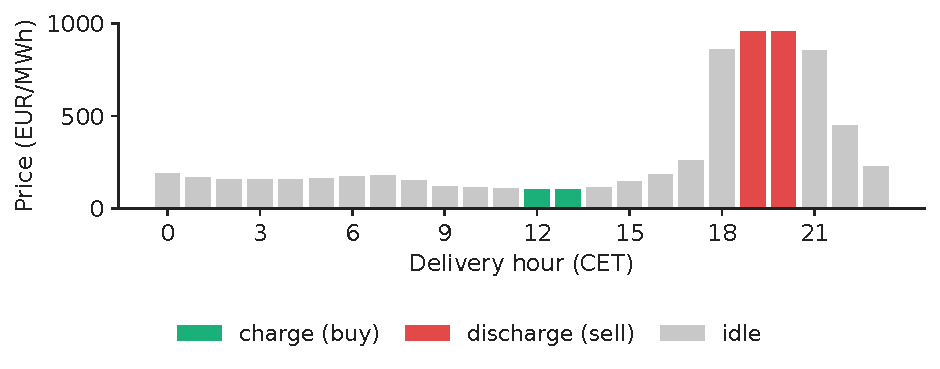
\includegraphics[width=\textwidth,height=0.417\textheight,keepaspectratio]{charts/en/dp_day.pdf}\end{center}\vspace{-3mm}
\chartsource{Source: energy-charts.info (Fraunhofer ISE), from exchange and ENTSO-E data. Data: Romania, 30 Jun 2026, hourly day-ahead prices.}
\vspace{0.5mm}
\begin{itemize}\setlength{\itemsep}{0pt}
  \item 30 Jun 2026: prices from 100.65 (hour 13) to 954.59 EUR/MWh (hour 20)
    \begin{itemize}\setlength{\itemsep}{0pt}
      \item 2 charging and 2 discharging hours.
    \end{itemize}
  \item Revenue of the day for a 2 MWh battery: 1\,541 EUR.
\end{itemize}
\par\vfill\noindent{\scriptsize\color{FooterGray}(own computation)}\hfill\qlink{NN\_L10\_dp\_day}{Quantlets/L10/NN_L10_dp_day}\par\vspace{0.5mm}
\end{frame}

\begin{frame}{The value function prices stored energy hour by hour}
\small
\intuition{$V_h(2)-V_h(0)$ is what two stored MWh are worth at hour $h$: high before the evening peak, zero after it.}
\begin{center}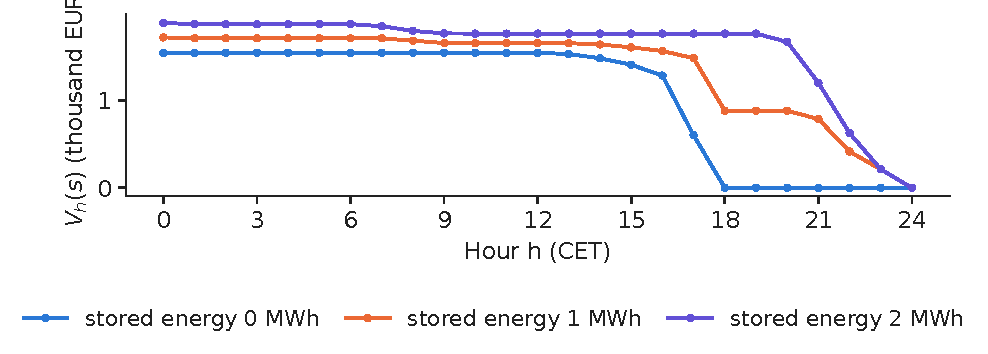
\includegraphics[width=\textwidth,height=0.401\textheight,keepaspectratio]{charts/en/dp_value.pdf}\end{center}\vspace{-3mm}
\chartsource{Source: energy-charts.info (Fraunhofer ISE), from exchange and ENTSO-E data. Data: Romania, 30 Jun 2026; own computation (backward induction).}
\vspace{0.5mm}
\begin{itemize}\setlength{\itemsep}{0pt}
  \item At 12:00 on 30 Jun 2026: $V_{12}(0)$ = 1\,541 EUR, $V_{12}(2)$ = 1\,760 EUR, so one stored MWh is worth 109.38 EUR, the shadow price of energy in the battery.
  \item A good learned $Q$ must reproduce this shape without seeing the day's prices.
\end{itemize}
\par\vfill\noindent{\scriptsize\color{FooterGray}(own computation)}\hfill\qlink{NN\_L10\_dp\_value}{Quantlets/L10/NN_L10_dp_value}\par\vspace{0.5mm}
\end{frame}

\begin{frame}{Perfect foresight: what a 2 MWh battery could have earned}
\small
\intuition{the DP revenue is an upper bound; it follows the spreads, not the price level.}
\begin{center}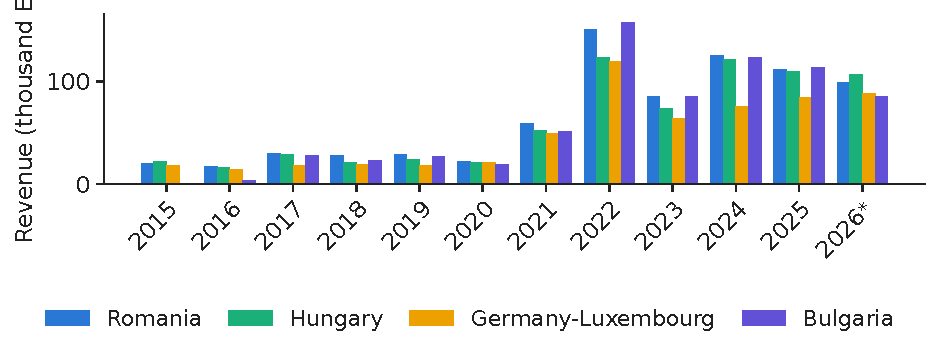
\includegraphics[width=\textwidth,height=0.357\textheight,keepaspectratio]{charts/en/dp_revenue_year.pdf}\end{center}\vspace{-3mm}
\chartsource{Source: energy-charts.info (Fraunhofer ISE), from exchange and ENTSO-E data. Data: 2015-2026 (*2026: January-October); days with 24 complete hours.}
\vspace{0.5mm}
\begin{itemize}\setlength{\itemsep}{0pt}
  \item Romania: 28.4 thousand EUR in 2019, 150.2 in 2022, 111.2 in 2025, 98.5 in 2026 over 302 days.
  \item 2025: Hungary 109.9, Bulgaria 112.9, Germany-Luxembourg 84.3 thousand EUR.
\end{itemize}
\par\vfill\manager{investors size storage on these numbers
    \begin{itemize}\setlength{\itemsep}{0pt}
      \item A real operator captures only part of them, as the next section measures.
    \end{itemize}}\par\vspace{0.5mm}
\par\vfill\noindent{\scriptsize\color{FooterGray}(own computation)}\hfill\qlink{NN\_L10\_dp\_revenue\_year}{Quantlets/L10/NN_L10_dp_revenue_year}\par\vspace{0.5mm}
\end{frame}


\section{Value-based learning: Q-learning and DQN}

\begin{frame}{Q-learning: learn $Q^{*}$ from samples, without a model}
\footnotesize
\intuition{move $Q(s,a)$ towards the reward plus the best value of the next state; the gap is the temporal-difference (TD) error.}
\begin{columns}[T,onlytextwidth]
\begin{column}{0.56\textwidth}
\[ Q(s_t,a_t)\leftarrow Q(s_t,a_t)+\alpha\,\underbrace{\big[r_{t+1}+\gamma\max_{a'}Q(s_{t+1},a')-Q(s_t,a_t)\big]}_{\text{TD error }\delta_t} \]{\footnotesize\begin{itemize}\setlength{\itemsep}{0pt}
  \item \textbf{\txtwhere}
    \begin{itemize}\setlength{\itemsep}{0pt}
      \item $\alpha$ = step size (0.05 here)
      \item The target uses the greedy action in $s_{t+1}$ whatever the agent does next, so Q-learning is \textbf{off-policy}.
    \end{itemize}
\end{itemize}\par}
\end{column}
\begin{column}{0.41\textwidth}
\begin{itemize}\setlength{\itemsep}{3pt}
  \item \textbf{Convergence} (Watkins \& Dayan, 1992): every pair $(s,a)$ visited infinitely often and $\sum\alpha_t=\infty$, $\sum\alpha_t^2<\infty$ (Appendix A).
  \item \textbf{Exploration}: $\varepsilon$-greedy
    \begin{itemize}\setlength{\itemsep}{0pt}
      \item Random action with probability $\varepsilon$, decayed from 1 to 0.05.
    \end{itemize}
  \item \textbf{Exploitation risk}: without exploration, a bad early estimate is never corrected.
\end{itemize}
\end{column}
\end{columns}
\par\vfill\manager{the TD error is a learning signal available after every hour, not only at the end of the day.}\par\vspace{0.5mm}
\par\vfill\noindent{\scriptsize\color{FooterGray}(Watkins \& Dayan, 1992)}\hfill\tryit{notebook \S3}\par\vspace{0.5mm}
\end{frame}

\begin{frame}{A realistic state: the agent sees yesterday, not today}
\footnotesize
\intuition{the operator plans before the day-ahead prices are known; the agent conditions on how cheap each hour was yesterday.}
\begin{columns}[T,onlytextwidth]
\begin{column}{0.55\textwidth}
\[ s_h=\big(h,\ \text{stored}_h,\ q_{h}\big),\quad q_h=\Big\lfloor\tfrac{\mathrm{rank}(p^{\,\text{yesterday}}_h)}{6}\Big\rfloor\in\{0,1,2,3\} \]{\footnotesize\begin{itemize}\setlength{\itemsep}{0pt}
  \item \textbf{\txtwhere}
    \begin{itemize}\setlength{\itemsep}{0pt}
      \item Rank of hour $h$ among yesterday's 24 prices, so $q_h=0$ = one of yesterday's six cheapest hours
      \item Table size $24\times4\times3$ states $\times$ 3 actions.
    \end{itemize}
\end{itemize}\par}
\end{column}
\begin{column}{0.42\textwidth}
\begin{itemize}\setlength{\itemsep}{3pt}
  \item \textbf{Training}: 1\,746 days of 2019--2023, 40 passes, the epoch with the best 2024 validation revenue is kept.
  \item \textbf{Test}: 638 days, 1 Jan 2025 -- 24 Oct 2026, used once.
  \item \textbf{Reward scale}: EUR/100, $\gamma=1$ within the day.
\end{itemize}
\end{column}
\end{columns}
\par\vfill\manager{a state that leaks today's prices would give a perfect but useless backtest.}\par\vspace{0.5mm}
\par\vfill\noindent{\scriptsize\color{FooterGray}(own computation)}\hfill\tryit{notebook \S3}\par\vspace{0.5mm}
\end{frame}

\begin{frame}{What tabular Q-learning learned}
\small
\intuition{with 1 MWh stored, the agent charges in hours that were cheap yesterday and sells in the evening.}
\begin{center}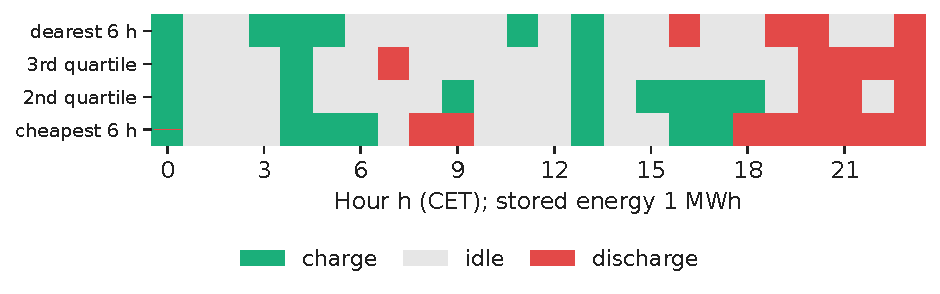
\includegraphics[width=\textwidth,height=0.417\textheight,keepaspectratio]{charts/en/q_policy.pdf}\end{center}\vspace{-3mm}
\chartsource{Source: energy-charts.info (Fraunhofer ISE), from exchange and ENTSO-E data. Data: rows = quartile of the hour's price yesterday; seed 20261108.}
\vspace{0.5mm}
\begin{itemize}\setlength{\itemsep}{0pt}
  \item A readable policy: the table can be printed and audited hour by hour (288 states).
  \item The hour of the day dominates
    \begin{itemize}\setlength{\itemsep}{0pt}
      \item Yesterday's ranking shifts the timing of charging.
    \end{itemize}
\end{itemize}
\par\vfill\noindent{\scriptsize\color{FooterGray}(own computation)}\hfill\qlink{NN\_L10\_q\_policy}{Quantlets/L10/NN_L10_q_policy}\par\vspace{0.5mm}
\end{frame}

\begin{frame}{From a table to a network: the deep Q-network}
\footnotesize
\intuition{replace the table by a network $Q_{\btheta}(s,a)$ and regress it on the TD target.}
\begin{columns}[T,onlytextwidth]
\begin{column}{0.56\textwidth}
\[ y=r+\gamma\,Q_{\btheta^{-}}\big(s',\argmax_{a'}Q_{\btheta}(s',a')\big) \]\[ \loss(\btheta)=\E_{(s,a,r,s')\sim\mathcal{D}}\big[\ell_{\text{Huber}}\big(y-Q_{\btheta}(s,a)\big)\big] \]{\footnotesize\begin{itemize}\setlength{\itemsep}{0pt}
  \item \textbf{\txtwhere}
    \begin{itemize}\setlength{\itemsep}{0pt}
      \item $\mathcal{D}$ = replay memory (the last four epochs)
      \item $\btheta^{-}$ = target network, a slow copy $\btheta^{-}\leftarrow(1-\tau)\btheta^{-}+\tau\btheta$, $\tau=0.005$
      \item Double DQN: the online network chooses $a'$, the target network evaluates it.
    \end{itemize}
\end{itemize}\par}
\end{column}
\begin{column}{0.41\textwidth}
\begin{itemize}\setlength{\itemsep}{3pt}
  \item \textbf{Replay} breaks the correlation of consecutive hours (Mnih et al., 2015).
  \item \textbf{Double DQN} removes the upward bias of $\max_{a'}$ over noisy estimates (van Hasselt et al., 2016).
  \item \textbf{Our network}: 82 inputs (yesterday's and last week's 24 standardised prices, weekday, hour, stored energy), two layers of 128 rectified linear units (ReLU), 3 outputs.
\end{itemize}
\end{column}
\end{columns}
\par\vfill\manager{function approximation + bootstrapping + off-policy data can diverge
    \begin{itemize}\setlength{\itemsep}{0pt}
      \item Replay and target networks keep it stable.
    \end{itemize}}\par\vspace{0.5mm}
\par\vfill\noindent{\scriptsize\color{FooterGray}(Mnih et al., 2015; van Hasselt, Guez \& Silver, 2016)}\hfill\tryit{notebook \S4}\par\vspace{0.5mm}
\end{frame}

\begin{frame}{Learning curves: validation revenue by training epoch}
\small
\intuition{both agents improve quickly but stay below yesterday's plan; the epoch kept is the best on 2024, never on the test years.}
\begin{center}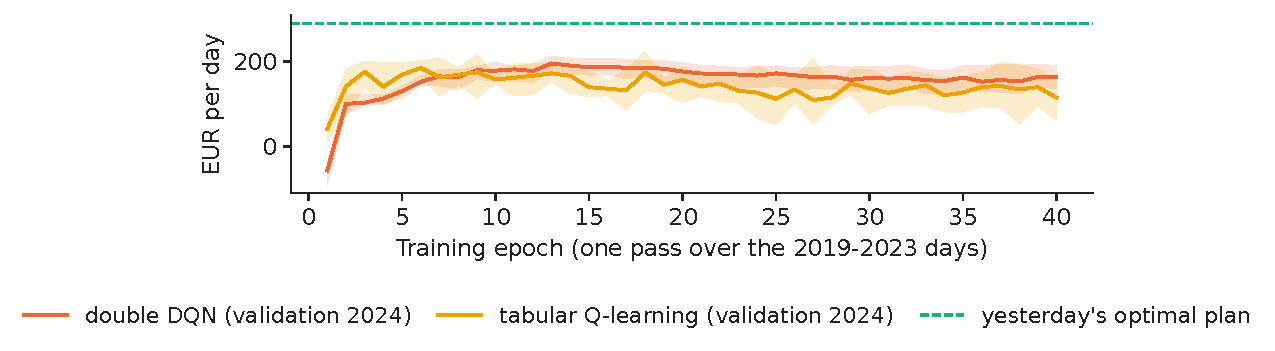
\includegraphics[width=\textwidth,height=0.453\textheight,keepaspectratio]{charts/en/battery_learning.pdf}\end{center}\vspace{-3mm}
\chartsource{Source: energy-charts.info (Fraunhofer ISE), from exchange and ENTSO-E data. Data: validation year 2024; band = range over 5 seeds.}
\vspace{0.5mm}
\begin{itemize}\setlength{\itemsep}{0pt}
  \item Best validation revenue per day, mean of 5 seeds: DQN 200 EUR, Q-learning 211 EUR, yesterday's plan 289 EUR.
\end{itemize}
\par\vfill\noindent{\scriptsize\color{FooterGray}(own computation)}\hfill\qlink{NN\_L10\_battery\_learning}{Quantlets/L10/NN_L10_battery_learning}\par\vspace{0.5mm}
\end{frame}

\begin{frame}{Test years: how much of the perfect-foresight revenue is captured}
\small
\intuition{cumulative revenue from 1 Jan 2025 to 24 Oct 2026; the gap to the top line is the value of perfect information.}
\begin{center}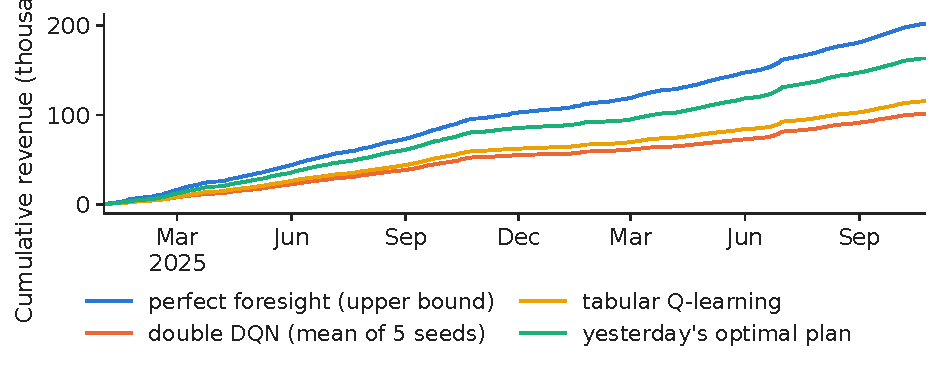
\includegraphics[width=\textwidth,height=0.391\textheight,keepaspectratio]{charts/en/battery_test_cum.pdf}\end{center}\vspace{-3mm}
\chartsource{Source: energy-charts.info (Fraunhofer ISE), from exchange and ENTSO-E data. Data: 1 Jan 2025 to 24 Oct 2026 (test); trained on 2019-2023, validated on 2024.}
\vspace{0.5mm}
\begin{itemize}\setlength{\itemsep}{0pt}
  \item Perfect foresight 202.1
    \begin{itemize}\setlength{\itemsep}{0pt}
      \item DQN 101.3
      \item Q-learning 115.2
      \item Yesterday's plan 163.1 thousand EUR.
    \end{itemize}
\end{itemize}
\par\vfill\noindent{\scriptsize\color{FooterGray}(own computation)}\hfill\qlink{NN\_L10\_battery\_test\_cum}{Quantlets/L10/NN_L10_battery_test_cum}\par\vspace{0.5mm}
\end{frame}

\begin{frame}{Battery results on the test years, five seeds}
\small
{\small\renewcommand{\arraystretch}{1.05}\setlength{\tabcolsep}{4pt}
\begin{tabular}{@{}p{0.36\textwidth}rrr@{}}\toprule
Strategy & Revenue (k EUR) & Capture (\%) & Seed range (\%) \\ \midrule
Perfect foresight (DP, upper bound) & 202.1 & 100 & -- \\
Double DQN & 101.3 & 50.1 & 43.9 -- 58.5 \\
Tabular Q-learning & 115.2 & 57.0 & 50.2 -- 61.9 \\
Yesterday's optimal plan (naive) & 163.1 & 80.7 & -- \\
\bottomrule\end{tabular}}\vspace{2mm}\begin{itemize}\setlength{\itemsep}{2pt}
  \item \textbf{Test of DQN against the naive plan}: daily revenue differences, Diebold-Mariano (DM) statistic with Newey-West variance (7 lags): $t$ = \ensuremath{-}18.99, $p$ = 0.000
    \begin{itemize}\setlength{\itemsep}{0pt}
      \item Mean difference \ensuremath{-}96.8 EUR per day.
    \end{itemize}
  \item DQN beats the naive plan in 0 of 5 seeds, Q-learning in 0 of 5: here the simple rule wins, because it optimises on all 24 of yesterday's prices, while the agents learn one average policy from a compressed state.
\end{itemize}
\par\vfill\manager{report the capture ratio with its range over seeds and a test against the naive plan, never a single best run.}\par\vspace{0.5mm}
\par\vfill\noindent{\scriptsize\color{FooterGray}(Diebold \& Mariano, 1995; own computation)}\hfill\tryit{notebook \S4}\par\vspace{0.5mm}
\end{frame}


\section{Policy gradients and PPO: trading the S\&P 500}

\begin{frame}{Policy gradient: push up the probability of actions that paid}
\footnotesize
\intuition{parameterise the policy directly and climb the gradient of the expected return.}
\begin{columns}[T,onlytextwidth]
\begin{column}{0.55\textwidth}
\[ \nabla_{\btheta}J(\btheta)=\E_{\pi_{\btheta}}\Big[\sum_{t}\nabla_{\btheta}\log\pi_{\btheta}(a_t\mid s_t)\,\big(G_t-b(s_t)\big)\Big] \]{\footnotesize\begin{itemize}\setlength{\itemsep}{0pt}
  \item \textbf{\txtwhere}
    \begin{itemize}\setlength{\itemsep}{0pt}
      \item $J(\btheta)=\E_{\pi_{\btheta}}[G_0]$
      \item $\nabla\log\pi$ = score function
      \item $b(s_t)$ = baseline, any function of the state, that leaves the gradient unbiased and lowers its variance
      \item $b=V_{\boldsymbol{\phi}}(s_t)$ gives an actor-critic.
    \end{itemize}
\end{itemize}\par}
\end{column}
\begin{column}{0.42\textwidth}
\begin{itemize}\setlength{\itemsep}{3pt}
  \item \textbf{REINFORCE} (Williams, 1992): Monte Carlo $G_t$
    \begin{itemize}\setlength{\itemsep}{0pt}
      \item Unbiased, high variance.
    \end{itemize}
  \item \textbf{Policy gradient theorem} (Sutton et al., 2000): the gradient needs no derivative of the transition law, so the market can stay a black box.
  \item \textbf{Stochastic policies} explore by themselves and handle continuous actions.
\end{itemize}
\end{column}
\end{columns}
\par\vfill\manager{the log-likelihood trick is the same one used to train classifiers, weighted by how good the outcome was.}\par\vspace{0.5mm}
\par\vfill\noindent{\scriptsize\color{FooterGray}(Williams, 1992; Sutton et al., 2000)}\par\vspace{0.5mm}
\end{frame}

\begin{frame}{Actor-critic and the advantage estimate}
\footnotesize
\intuition{a critic $V_{\boldsymbol{\phi}}$ predicts the return, and the actor learns from the surprise $\hat A_t$.}
\begin{columns}[T,onlytextwidth]
\begin{column}{0.56\textwidth}
\[ \delta_t=r_{t+1}+\gamma V_{\boldsymbol{\phi}}(s_{t+1})-V_{\boldsymbol{\phi}}(s_t),\qquad \hat A_t=\sum_{l\ge0}(\gamma\lambda)^{l}\,\delta_{t+l} \]\[ \loss_V(\boldsymbol{\phi})=\E\big[(\hat A_t+V_{\boldsymbol{\phi}}^{\text{old}}(s_t)-V_{\boldsymbol{\phi}}(s_t))^2\big] \]{\footnotesize\begin{itemize}\setlength{\itemsep}{0pt}
  \item \textbf{\txtwhere}
    \begin{itemize}\setlength{\itemsep}{0pt}
      \item Generalised advantage estimation (GAE): $\lambda=0$ gives the one-step TD advantage (low variance, biased), $\lambda=1$ the Monte Carlo advantage
      \item We use $\gamma=0.99$, $\lambda=0.95$.
    \end{itemize}
\end{itemize}\par}
\end{column}
\begin{column}{0.41\textwidth}
\begin{itemize}\setlength{\itemsep}{3pt}
  \item \textbf{Shared body}: actor and critic share two layers of 64 tanh units
    \begin{itemize}\setlength{\itemsep}{0pt}
      \item Heads: 2 action logits and 1 value.
    \end{itemize}
  \item \textbf{Advantage normalisation} in each batch keeps the step size comparable across market regimes.
  \item \textbf{Entropy bonus} 0.01 keeps the policy from collapsing too early.
\end{itemize}
\end{column}
\end{columns}
\par\vfill\manager{the critic is a forecast of future reward
    \begin{itemize}\setlength{\itemsep}{0pt}
      \item A poor critic gives noisy advantages and slow learning.
    \end{itemize}}\par\vspace{0.5mm}
\par\vfill\noindent{\scriptsize\color{FooterGray}(Schulman et al., 2016)}\par\vspace{0.5mm}
\end{frame}

\begin{frame}{PPO: improve the policy, but not too far in one step}
\small
\intuition{the clipped objective removes the incentive to move the probability ratio outside $[1-\epsilon,1+\epsilon]$.}
\vspace{-1mm}\[ \loss^{\text{CLIP}}(\btheta)=\E_t\big[\min\big(\rho_t\hat A_t,\ \mathrm{clip}(\rho_t,1-\epsilon,1+\epsilon)\hat A_t\big)\big],\quad \rho_t=\frac{\pi_{\btheta}(a_t\mid s_t)}{\pi_{\btheta_{\text{old}}}(a_t\mid s_t)} \]\vspace{-2mm}
\begin{center}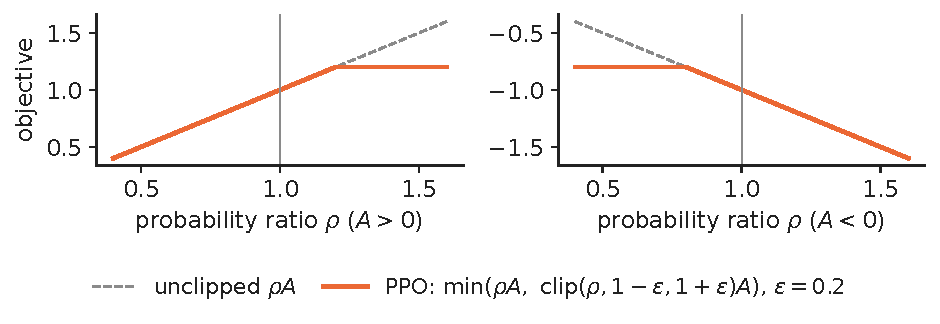
\includegraphics[width=\textwidth,height=0.364\textheight,keepaspectratio]{charts/en/ppo_clip.pdf}\end{center}\vspace{-3mm}
\chartsource{Source: Schulman et al. (2017), clipped surrogate objective. Data: analytic function, no data.}
\vspace{0.5mm}
\begin{itemize}\setlength{\itemsep}{0pt}
  \item \simlabel\ Analytic function, no data
    \begin{itemize}\setlength{\itemsep}{0pt}
      \item $\epsilon=0.2$
      \item A cheap substitute for the Kullback-Leibler (KL) trust region of trust region policy optimisation (TRPO).
    \end{itemize}
\end{itemize}
\par\vfill\noindent{\scriptsize\color{FooterGray}(Schulman et al., 2017)}\hfill\qlink{NN\_L10\_ppo\_clip}{Quantlets/L10/NN_L10_ppo_clip}\par\vspace{0.5mm}
\end{frame}

\begin{frame}{Trading as an MDP: flat or long the S\&P 500}
\footnotesize
\intuition{each evening the agent chooses tomorrow's position; it earns the next day's return and pays a cost when it changes position.}
\begin{columns}[T,onlytextwidth]
\begin{column}{0.53\textwidth}
\[ r_{t+1}=a_t\,\ln\frac{P_{t+1}}{P_t}-c\,|a_t-a_{t-1}|,\qquad a_t\in\{0,1\},\ c=5\ \text{bp} \]{\footnotesize\begin{itemize}\setlength{\itemsep}{0pt}
  \item \textbf{\txtwhere}
    \begin{itemize}\setlength{\itemsep}{0pt}
      \item $s_t$ = 7 features standardised on 2005--2016 (log returns over 1, 5, 21, 63 days, 21-day volatility, VIX, distance to the 200-day average) + $a_{t-1}$.
    \end{itemize}
\end{itemize}\par}
\end{column}
\begin{column}{0.44\textwidth}
\begin{itemize}\setlength{\itemsep}{2pt}
  \item \textbf{Training}: 150 PPO iterations of 64 random 126-day windows from 2005--2016, clip 0.2.
  \item \textbf{Selection}: the iteration with the best 2017--2019 Sharpe ratio.
  \item \textbf{Test}: 1\,716 days from 2 Jan 2020, five seeds, against buy-and-hold and the 200-day moving average.
\end{itemize}
\end{column}
\end{columns}
\par\vfill\manager{put the cost in the reward, or the agent trades far too often.}\par\vspace{0.5mm}
\par\vfill\noindent{\scriptsize\color{FooterGray}(Moody \& Saffell, 2001; own computation)}\hfill\tryit{notebook \S5}\par\vspace{0.5mm}
\end{frame}

\begin{frame}{Training and validation Sharpe ratios during PPO training}
\small
\intuition{the training Sharpe ratio rises; the validation ratio is noisy, and the best iteration is kept.}
\begin{center}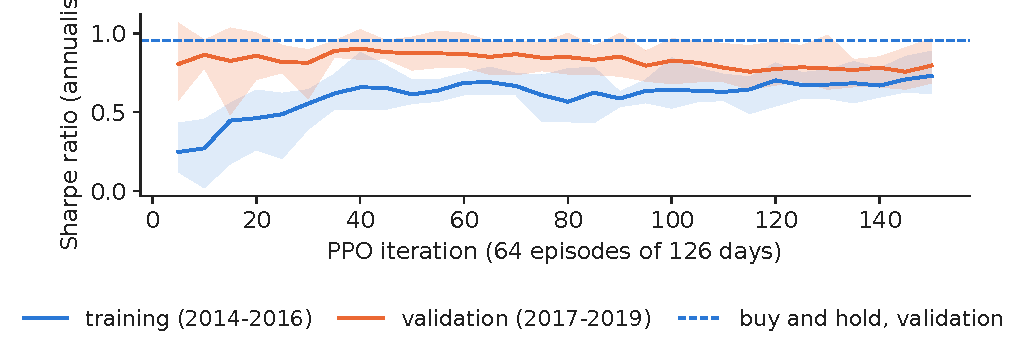
\includegraphics[width=\textwidth,height=0.500\textheight,keepaspectratio]{charts/en/trading_learning.pdf}\end{center}\vspace{-3mm}
\chartsource{Source: Yahoo Finance, daily quotes. Data: training windows from 17 Oct 2005 to 30 Dec 2016; band = range over 5 seeds.}
\vspace{0.5mm}
\begin{itemize}\setlength{\itemsep}{0pt}
  \item Buy-and-hold Sharpe on validation (2017--2019): 0.95
    \begin{itemize}\setlength{\itemsep}{0pt}
      \item The selected iteration is on average 48.
    \end{itemize}
\end{itemize}
\par\vfill\noindent{\scriptsize\color{FooterGray}(own computation)}\hfill\qlink{NN\_L10\_trading\_learning}{Quantlets/L10/NN_L10_trading_learning}\par\vspace{0.5mm}
\end{frame}

\begin{frame}{Test period: the PPO agent against two simple rules}
\small
\intuition{value of 1 USD invested on 2 Jan 2020, after a 5 basis-point cost per change of position.}
\begin{center}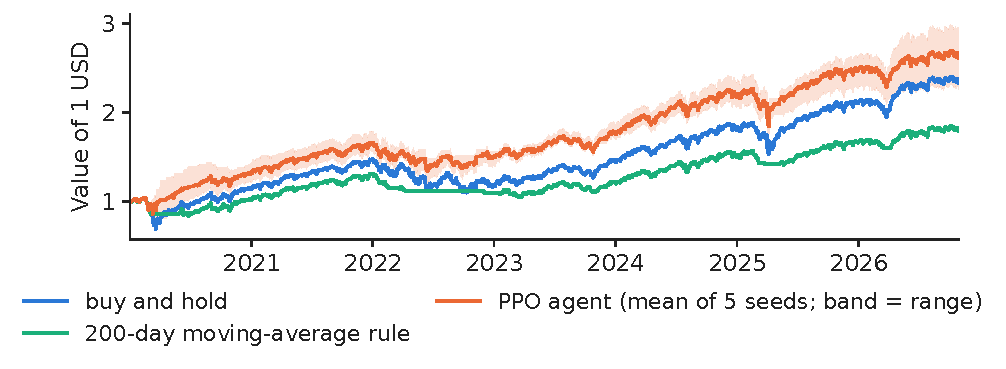
\includegraphics[width=\textwidth,height=0.467\textheight,keepaspectratio]{charts/en/trading_equity.pdf}\end{center}\vspace{-3mm}
\chartsource{Source: Yahoo Finance, daily quotes. Data: 2 Jan 2020 to 29 Oct 2026 (test), S\&P 500, 5 bp cost per trade.}
\vspace{0.5mm}
\begin{itemize}\setlength{\itemsep}{0pt}
  \item Sharpe ratio: buy-and-hold 0.61
    \begin{itemize}\setlength{\itemsep}{0pt}
      \item Moving-average rule 0.68
      \item PPO 0.83 (seeds from 0.72 to 0.95).
    \end{itemize}
\end{itemize}
\par\vfill\noindent{\scriptsize\color{FooterGray}(own computation)}\hfill\qlink{NN\_L10\_trading\_equity}{Quantlets/L10/NN_L10_trading_equity}\par\vspace{0.5mm}
\end{frame}

\begin{frame}{Trading results on the test period}
\small
{\small\renewcommand{\arraystretch}{1.05}\setlength{\tabcolsep}{4pt}
\begin{tabular}{@{}p{0.25\textwidth}rrrrrr@{}}\toprule
Strategy & Return \%/yr & Vol.\ \%/yr & Sharpe & Drawdown \% & Invested \% & Trades \\ \midrule
Buy and hold & 13.2 & 20.2 & 0.61 & \ensuremath{-}33.9 & 100 & 1 \\
200-day moving average & 8.9 & 12.4 & 0.68 & \ensuremath{-}20.5 & 79 & 41 \\
PPO (mean of 5 seeds) & 15.1 & 17.0 & 0.83 & \ensuremath{-}23.2 & 82 & 147 \\
\bottomrule\end{tabular}}\vspace{2mm}\begin{itemize}\setlength{\itemsep}{2pt}
  \item \textbf{Uncertainty}: Sharpe difference of the seed-averaged PPO strategy minus buy-and-hold \ensuremath{+}0.26
    \begin{itemize}\setlength{\itemsep}{0pt}
      \item 95\,\% stationary block-bootstrap interval [\ensuremath{-}0.08; 0.56] (2,000 resamples, mean block 21 days).
    \end{itemize}
  \item PPO beats buy-and-hold on the Sharpe ratio in 5 of 5 seeds.
\end{itemize}
\par\vfill\manager{an interval that contains zero means: no evidence that the agent adds value, whatever the backtest chart suggests.}\par\vspace{0.5mm}
\par\vfill\noindent{\scriptsize\color{FooterGray}(Politis \& Romano, 1994; own computation)}\hfill\tryit{notebook \S5}\par\vspace{0.5mm}
\end{frame}

\begin{frame}{When is the agent out of the market?}
\small
\intuition{exposure of the PPO agent (share of seeds and days invested) against the moving-average rule.}
\begin{center}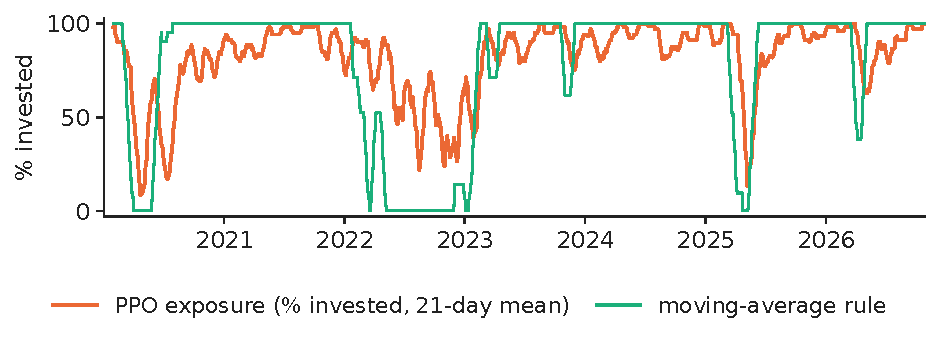
\includegraphics[width=\textwidth,height=0.346\textheight,keepaspectratio]{charts/en/trading_exposure.pdf}\end{center}\vspace{-3mm}
\chartsource{Source: Yahoo Finance, daily quotes. Data: 2 Jan 2020 to 29 Oct 2026 (test).}
\vspace{0.5mm}
\begin{itemize}\setlength{\itemsep}{0pt}
  \item Invested: PPO 82\,\% of test days
    \begin{itemize}\setlength{\itemsep}{0pt}
      \item 20 Feb -- 30 Apr 2020 42\,\% (moving average 14\,\%)
      \item 2022 63\,\% (moving average 15\,\%).
    \end{itemize}
\end{itemize}
\par\vfill\manager{read the policy, not only its profit: an agent that is simply always long is buy-and-hold with extra model risk.}\par\vspace{0.5mm}
\par\vfill\noindent{\scriptsize\color{FooterGray}(own computation)}\hfill\qlink{NN\_L10\_trading\_exposure}{Quantlets/L10/NN_L10_trading_exposure}\par\vspace{0.5mm}
\end{frame}

\begin{frame}{Why RL trading backtests mislead}
\small
\begin{itemize}\setlength{\itemsep}{4pt}
  \item \textbf{Low signal-to-noise}: daily equity returns are close to unpredictable
    \begin{itemize}\setlength{\itemsep}{0pt}
      \item The agent mostly learns the noise of its training windows.
    \end{itemize}
  \item \textbf{Non-stationarity}: 2005--2016 contains 2008
    \begin{itemize}\setlength{\itemsep}{0pt}
      \item 2020--2026 contains a pandemic crash, an inflation shock and a long rally.
    \end{itemize}
  \item \textbf{Seed and selection risk}: five seeds already give a range of Sharpe ratios
    \begin{itemize}\setlength{\itemsep}{0pt}
      \item Reporting the best seed is backtest overfitting.
    \end{itemize}
  \item \textbf{Price impact and costs}: a price-taking simulator ignores market impact
    \begin{itemize}\setlength{\itemsep}{0pt}
      \item Costs must be in the reward, not added afterwards.
    \end{itemize}
  \item \textbf{Where RL helps more}: execution (splitting a large order), market making, hedging, storage: problems with a real state and a known reward.
\end{itemize}
\par\vfill\manager{ask for the seed distribution, the cost assumption and a bootstrap interval before trusting any RL trading result.}\par\vspace{0.5mm}
\par\vfill\noindent{\scriptsize\color{FooterGray}(Hambly, Xu \& Yang, 2023)}\par\vspace{0.5mm}
\end{frame}


\section{Deep hedging: a policy that minimises tail risk}

\begin{frame}{Hedging a short call: the profit and loss of the desk}
\footnotesize
\intuition{the desk sells a one-month at-the-money (ATM) call and trades the index every day to offset the risk.}
\begin{columns}[T,onlytextwidth]
\begin{column}{0.56\textwidth}
\[ \mathrm{PL}(\delta)=C_0+\sum_{k=0}^{20}\delta_k\,(S_{k+1}-S_k)-(S_{21}-K)^{+}-c\sum_{k=0}^{21}S_k\,|\delta_k-\delta_{k-1}| \]{\footnotesize\begin{itemize}\setlength{\itemsep}{0pt}
  \item \textbf{\txtwhere}
    \begin{itemize}\setlength{\itemsep}{0pt}
      \item $S_k$ = S\&P 500 close on day $k$ of a real 21-day path, $S_0=K=1$
      \item $C_0$ = Black-Scholes premium (VIX of day 0, rate 0), $\delta_k$ = units held over $(k,k+1]$, $c$ = 10 bp.
    \end{itemize}
\end{itemize}\par}
\end{column}
\begin{column}{0.41\textwidth}
\begin{itemize}\setlength{\itemsep}{2pt}
  \item \textbf{Paths}: one per start day
    \begin{itemize}\setlength{\itemsep}{0pt}
      \item Training 3\,021 (2005--2016), validation 754, test 1\,696 paths from 2020.
    \end{itemize}
  \item \textbf{Test}: mean premium 2.38\,\%, mean payoff 2.53\,\% of the index (mean VIX 20.7).
  \item \textbf{Real, not simulated}: the paths keep the jumps and volatility clusters of 2008, 2020 and 2022.
\end{itemize}
\end{column}
\end{columns}
\par\vfill\manager{the premium barely covers the mean payoff
    \begin{itemize}\setlength{\itemsep}{0pt}
      \item The risk desk manages the tail.
    \end{itemize}}\par\vspace{0.5mm}
\par\vfill\noindent{\scriptsize\color{FooterGray}(Buehler et al., 2019)}\hfill\tryit{notebook \S6}\par\vspace{0.5mm}
\end{frame}

\begin{frame}{Black-Scholes delta and the deep-hedging objective}
\footnotesize
\intuition{the benchmark hedges the model sensitivity; the network instead minimises the expected shortfall of the real loss, costs included.}
\begin{columns}[T,onlytextwidth]
\begin{column}{0.56\textwidth}
\[ \delta_k^{\text{BS}}=\Phi(d_1),\quad d_1=\frac{\ln(S_k/K)+\tfrac12\sigma_k^{2}\tau_k}{\sigma_k\sqrt{\tau_k}} \]\[ \min_{\btheta,w}\ w+\frac{1}{1-\alpha}\E\big[(-\mathrm{PL}(\delta_{\btheta})-w)^{+}\big]=\min_{\btheta}\mathrm{ES}_{\alpha}\big(-\mathrm{PL}(\delta_{\btheta})\big) \]{\footnotesize\begin{itemize}\setlength{\itemsep}{0pt}
  \item \textbf{\txtwhere}
    \begin{itemize}\setlength{\itemsep}{0pt}
      \item $\sigma_k$ = VIX/100, $\tau_k=(21-k)/252$, $\alpha=0.95$
      \item At the optimum $w$ is the value at risk (VaR)
      \item $\delta_{\btheta}(\ln S_k,\tau_k,\sigma_k,\delta_{k-1})\in[0,1]$: 2 layers of 32 ReLU units, sigmoid output.
    \end{itemize}
\end{itemize}\par}
\end{column}
\begin{column}{0.41\textwidth}
\begin{itemize}\setlength{\itemsep}{3pt}
  \item \textbf{Policy optimisation with a known reward}: the profit and loss is differentiable in $\btheta$, so we back-propagate through all 21 days.
  \item \textbf{Previous hedge as input}: lets the network learn a no-trade band when costs are high.
  \item \textbf{Training}: 600 full-batch Adam steps, five seeds.
\end{itemize}
\end{column}
\end{columns}
\par\vfill\manager{the objective is the risk measure the desk reports.}\par\vspace{0.5mm}
\par\vfill\noindent{\scriptsize\color{FooterGray}(Buehler et al., 2019; Rockafellar \& Uryasev, 2000)}\hfill\tryit{notebook \S6}\par\vspace{0.5mm}
\end{frame}

\begin{frame}{Hedging profit and loss on the test paths}
\small
\intuition{hedging removes most of the left tail; the deep hedge cuts the remaining tail further, at lower turnover.}
\begin{center}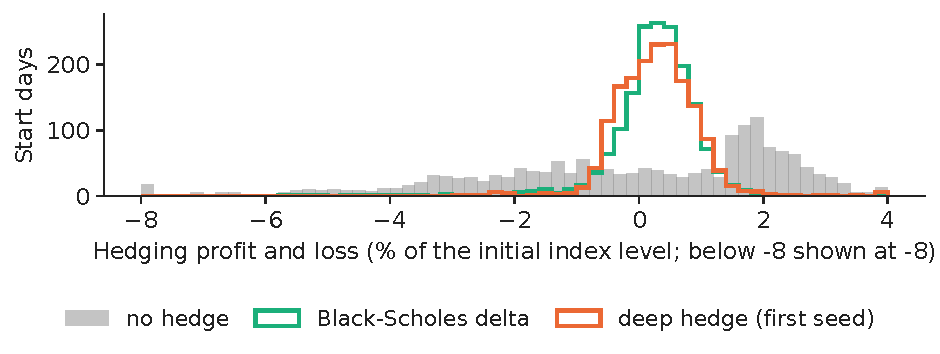
\includegraphics[width=\textwidth,height=0.520\textheight,keepaspectratio]{charts/en/hedge_pnl.pdf}\end{center}\vspace{-3mm}
\chartsource{Source: Yahoo Finance, daily quotes. Data: 21-day paths starting 2 Jan 2020 to 1 Oct 2026 (test); S\&P 500 and VIX; 10 bp cost.}
\vspace{0.5mm}
\begin{itemize}\setlength{\itemsep}{0pt}
  \item Standard deviation: no hedge 2.60, delta 0.74, deep hedge 0.69 (\% of the index).
\end{itemize}
\par\vfill\noindent{\scriptsize\color{FooterGray}(own computation)}\hfill\qlink{NN\_L10\_hedge\_pnl}{Quantlets/L10/NN_L10_hedge_pnl}\par\vspace{0.5mm}
\end{frame}

\begin{frame}{Hedging results on the test paths, 10 bp cost}
\small
{\small\renewcommand{\arraystretch}{1.05}\setlength{\tabcolsep}{4pt}
\begin{tabular}{@{}p{0.34\textwidth}rrrr@{}}\toprule
Strategy & Mean PL (\%) & Std.\ dev.\ (\%) & ES$_{95}$ of loss (\%) & Turnover \\ \midrule
No hedge & \ensuremath{-}0.15 & 2.60 & 6.82 & 0 \\
Black-Scholes delta (VIX) & 0.24 & 0.74 & 1.94 & 1.71 \\
Deep hedge (mean of 5 seeds) & 0.27 & 0.69 & 1.15 & 1.32 \\
\bottomrule\end{tabular}}\vspace{2mm}\begin{itemize}\setlength{\itemsep}{2pt}
  \item ES$_{95}$ of the deep hedge across seeds: 1.10 -- 1.24
    \begin{itemize}\setlength{\itemsep}{0pt}
      \item Lower than the delta hedge in 5 of 5 seeds.
    \end{itemize}
  \item PL = profit and loss in \% of the initial index level
    \begin{itemize}\setlength{\itemsep}{0pt}
      \item Turnover = mean $\sum_k|\delta_k-\delta_{k-1}|$ per path.
    \end{itemize}
\end{itemize}
\par\vfill\manager{judge a hedge by the tail of the loss and by its turnover, not by its mean profit.}\par\vspace{0.5mm}
\par\vfill\noindent{\scriptsize\color{FooterGray}(own computation)}\hfill\tryit{notebook \S6}\par\vspace{0.5mm}
\end{frame}

\begin{frame}{What the network learned: a flatter, cost-aware hedge ratio}
\small
\intuition{hedge ratio as a function of moneyness, 10 days before maturity, with the VIX at 20.}
\begin{center}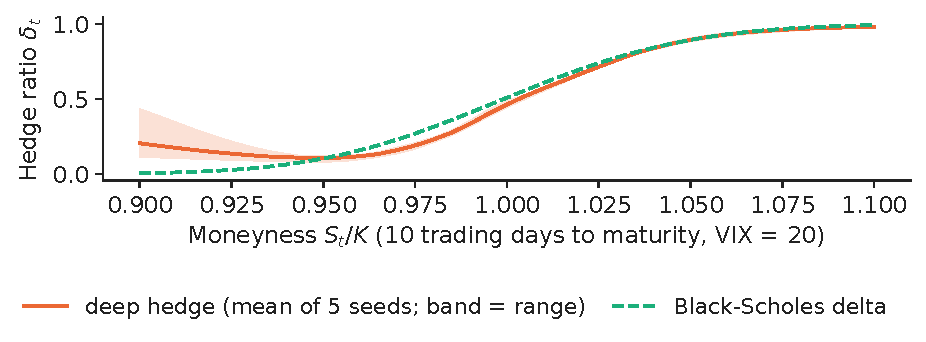
\includegraphics[width=\textwidth,height=0.500\textheight,keepaspectratio]{charts/en/hedge_delta.pdf}\end{center}\vspace{-3mm}
\chartsource{Source: Yahoo Finance, daily quotes. Data: policy trained on 21-day paths starting 2005-2016.}
\vspace{0.5mm}
\begin{itemize}\setlength{\itemsep}{0pt}
  \item At the money: deep hedge 0.46 against Black-Scholes 0.51
    \begin{itemize}\setlength{\itemsep}{0pt}
      \item The band shows the spread across five seeds.
    \end{itemize}
\end{itemize}
\par\vfill\noindent{\scriptsize\color{FooterGray}(own computation)}\hfill\qlink{NN\_L10\_hedge\_delta}{Quantlets/L10/NN_L10_hedge_delta}\par\vspace{0.5mm}
\end{frame}

\begin{frame}{Transaction costs: where the learned hedge helps}
\small
\intuition{ES$_{95}$ of the hedging loss for cost levels from 0 to 50 bp; one network trained per cost level.}
\begin{center}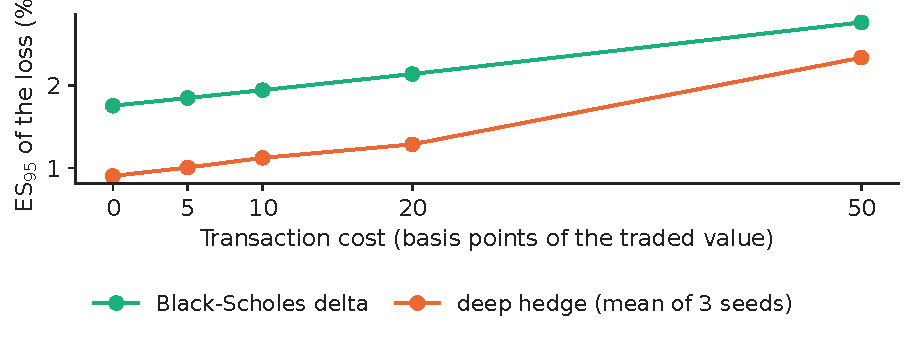
\includegraphics[width=\textwidth,height=0.388\textheight,keepaspectratio]{charts/en/hedge_costs.pdf}\end{center}\vspace{-3mm}
\chartsource{Source: Yahoo Finance, daily quotes. Data: test paths starting 2 Jan 2020 to 1 Oct 2026.}
\vspace{0.5mm}
\begin{itemize}\setlength{\itemsep}{0pt}
  \item No cost: delta 1.75, deep hedge 0.90
    \begin{itemize}\setlength{\itemsep}{0pt}
      \item 50 bp: delta 2.76, deep hedge 2.34 (\% of the index).
    \end{itemize}
\end{itemize}
\par\vfill\manager{the value of a learned hedge grows with frictions: illiquid underlyings, wide spreads, energy and commodity hedges.}\par\vspace{0.5mm}
\par\vfill\noindent{\scriptsize\color{FooterGray}(own computation)}\hfill\qlink{NN\_L10\_hedge\_costs}{Quantlets/L10/NN_L10_hedge_costs}\par\vspace{0.5mm}
\end{frame}

\begin{frame}{Reinforcement learning in production: model risk}
\small
\begin{columns}[T,onlytextwidth]
\begin{column}{0.49\textwidth}
\begin{itemize}\setlength{\itemsep}{4pt}
  \item \textbf{Reward design}: the agent optimises exactly what you write
    \begin{itemize}\setlength{\itemsep}{0pt}
      \item Omit costs, risk or constraints and it will exploit the gap.
    \end{itemize}
  \item \textbf{Simulator gap}: a historical replay ignores the agent's own price impact and future regimes.
  \item \textbf{Offline evaluation}: one test period used once
    \begin{itemize}\setlength{\itemsep}{0pt}
      \item Several seeds
      \item A test against the rule in use.
    \end{itemize}
\end{itemize}
\end{column}
\begin{column}{0.49\textwidth}
\begin{itemize}\setlength{\itemsep}{4pt}
  \item \textbf{Guardrails}: action masks (state of charge, position limits), kill switches, human sign-off.
  \item \textbf{Explainability}: a table or a hedge-ratio curve can be audited
    \begin{itemize}\setlength{\itemsep}{0pt}
      \item Lecture 11 explains neural policies.
    \end{itemize}
  \item \textbf{Monitoring}: compare live capture ratio and turnover with the backtest every month.
\end{itemize}
\end{column}
\end{columns}
\par\vfill\manager{treat an RL policy like any model of the bank: documented, validated independently, monitored, with a fallback rule.}\par\vspace{0.5mm}
\par\vfill\noindent{\scriptsize\color{FooterGray}(Hambly, Xu \& Yang, 2023)}\par\vspace{0.5mm}
\end{frame}

\section*{Wrap-up}

\begin{frame}{Quiz 1: perfect foresight}
\small
\begin{itemize}
  \item A vendor shows that its battery agent earned 95\,\% of the dynamic-programming revenue in a backtest in which the DP used the day's own prices.
    \begin{itemize}\setlength{\itemsep}{0pt}
      \item What do you ask?
    \end{itemize}
\end{itemize}
\vspace{2mm}
\begin{exampleblock}{Answer}
\begin{itemize}
  \item Whether the agent's state contained the day's prices: if so, the 95\,\% is look-ahead bias
    \begin{itemize}\setlength{\itemsep}{0pt}
      \item A fair agent sees only yesterday and is compared with yesterday's optimal plan, as in our test (DQN 50.1\,\%, naive 80.7\,\%).
    \end{itemize}
\end{itemize}
\end{exampleblock}
\end{frame}

\begin{frame}{Quiz 2: PPO clipping}
\small
\begin{itemize}
  \item In a PPO update an action has advantage $\hat A_t>0$ and the new policy already gives it 1.5 times its old probability.
    \begin{itemize}\setlength{\itemsep}{0pt}
      \item What gradient does the clipped objective pass to this sample with $\epsilon=0.2$?
    \end{itemize}
\end{itemize}
\vspace{2mm}
\begin{exampleblock}{Answer}
\begin{itemize}
  \item Zero: $\rho_t=1.5>1+\epsilon$, the minimum picks the clipped term $1.2\,\hat A_t$, which does not depend on $\btheta$
    \begin{itemize}\setlength{\itemsep}{0pt}
      \item The policy is not pushed further in this step.
    \end{itemize}
\end{itemize}
\end{exampleblock}
\end{frame}

\begin{frame}{Quiz 3: reading a trading result}
\small
\begin{itemize}
  \item Your PPO agent shows a test Sharpe ratio above buy-and-hold for its best seed.
    \begin{itemize}\setlength{\itemsep}{0pt}
      \item The bootstrap interval of the Sharpe difference of the seed-averaged strategy is [\ensuremath{-}0.08; 0.56].
      \item Do you deploy it?
    \end{itemize}
\end{itemize}
\vspace{2mm}
\begin{exampleblock}{Answer}
\begin{itemize}
  \item No: the best seed is a selected outcome, and an interval that contains zero gives no evidence of added value
    \begin{itemize}\setlength{\itemsep}{0pt}
      \item Keep the simple rule.
    \end{itemize}
\end{itemize}
\end{exampleblock}
\end{frame}

\begin{frame}{Wrap-up}
\small
\begin{itemize}\setlength{\itemsep}{4pt}
  \item \textbf{MDP + Bellman}: write state, action, reward
    \begin{itemize}\setlength{\itemsep}{0pt}
      \item DP solves small problems exactly and gives the ceiling (battery: 202.1 thousand EUR on the test years).
    \end{itemize}
  \item \textbf{Value-based}: Q-learning and DQN learn from yesterday's prices
    \begin{itemize}\setlength{\itemsep}{0pt}
      \item Capture ratios 57.0\,\% and 50.1\,\%, naive plan 80.7\,\%.
    \end{itemize}
  \item \textbf{Policy gradient}: PPO on the S\&P 500 gives a Sharpe ratio of 0.83 against 0.61 for buy-and-hold, with a bootstrap interval that contains zero.
  \item \textbf{Deep hedging}: ES$_{95}$ of the loss 1.15\,\% against 1.94\,\% for the delta hedge at 10 bp.
  \item \textbf{Verdict on real data}: battery --- the simple rule wins
    \begin{itemize}\setlength{\itemsep}{0pt}
      \item Trading --- higher Sharpe, but not significant
      \item Hedging --- the learned policy wins in every seed.
    \end{itemize}
  \item \textbf{Next}: Lecture 11 opens the black box: explaining what a neural network has learned.
\end{itemize}
\end{frame}

\begin{frame}{Research from our group: storage, prices and learning in energy finance}
\footnotesize
\begin{itemize}\setlength{\itemsep}{4pt}
  \item \textbf{Battery arbitrage on day-ahead markets}: joint probabilistic forecasts of the hourly price vector feed the charge-discharge decision of a battery in Central and Eastern European day-ahead markets
    \begin{itemize}\setlength{\itemsep}{0pt}
      \item Forecasting the joint distribution, not only point prices, is what the dispatch needs (Andrei, Cepoi, Dumitrescu, Lessmann, Chiriac (Luchian), Pele \& Petukhina, 2026, Social Science Research Network (SSRN) 6872381).
    \end{itemize}
  \item \textbf{Four generations of price models}: a comparative evaluation from statistical models to machine learning, deep learning and transformer models for energy prices (Andrei, Velev, Toma, Pele \& Lessmann, 2024, arXiv 2411.03372) --- the forecasts a dispatch agent consumes.
  \item \textbf{Artificial intelligence (AI) in energy finance}: a systematic literature review of how machine learning and reinforcement learning reshape trading, risk and storage decisions in energy markets (Anagnoste et al., 2025, Energy Strategy Reviews).
\end{itemize}\par\vspace{1mm}{\scriptsize \begin{itemize}
  \item Findings as stated in the papers; numbers on the other slides come from our own data.
\end{itemize}}
\par\vfill\noindent{\scriptsize\color{FooterGray}(Bucharest University of Economic Studies (ASE); Romanian Academy, Institute for Economic Forecasting (IPE))}\par\vspace{0.5mm}
\end{frame}

\begin{frame}{Want to learn more?}
\small
\begin{columns}[T,onlytextwidth]
\begin{column}{0.5\textwidth}
\begin{itemize}\setlength{\itemsep}{4pt}
  \item \textbf{Sutton \& Barto (2018)}, the reference text, free online: \href{http://incompleteideas.net/book/the-book-2nd.html}{incompleteideas.net/book}.
  \item \textbf{Spinning Up in Deep RL} (OpenAI), clear derivations of policy gradients and PPO: \href{https://spinningup.openai.com}{spinningup.openai.com}.
  \item \textbf{Hambly, Xu \& Yang (2023)}: survey of RL in finance.
\end{itemize}
\end{column}
\begin{column}{0.47\textwidth}
\begin{itemize}\setlength{\itemsep}{4pt}
  \item \textbf{This course}: code, data, notebooks --- \href{https://github.com/danpele/NEURAL_BIZ}{github.com/danpele/NEURAL\_BIZ}.
  \item \textbf{Experiment yourself}: notebooks/L10\_notebook.ipynb reproduces every method of this lecture
    \begin{itemize}\setlength{\itemsep}{0pt}
      \item The seminar adds efficiency, battery size and cost experiments.
    \end{itemize}
  \item \textbf{Deep hedging}: Buehler et al.\ (2019), the paper behind the last section.
\end{itemize}
\end{column}
\end{columns}
\end{frame}

\begin{frame}{References (1/2)}
\scriptsize
\begin{itemize}\setlength{\itemsep}{0pt}\scriptsize
\item Andrei, A.-V., Cepoi, C.\,O., Dumitrescu, B.\,A., Lessmann, S., Chiriac (Luchian), A.-C., Pele, D.\,T.\ \& Petukhina, A.\ (2026). Joint probabilistic forecasting for battery arbitrage in day-ahead power markets. SSRN Working Paper 6872381. \href{https://doi.org/10.2139/ssrn.6872381}{doi:10.2139/ssrn.6872381}
\item Anagnoste, S., Andrei, A.-V., Bolovăneanu, V., Cepoi, C.-O., Clodnitchi, R., Cramer, A.-A., Grecu, R.-A., Lessmann, S., Pele, D.\,T., Petukhina, A.\ \& Strat, V.\,A.\ (2025). The role of AI in (re)shaping energy finance: A systematic literature review. \textit{Energy Strategy Reviews}, 61, 101833. \href{https://doi.org/10.1016/j.esr.2025.101833}{doi:10.1016/j.esr.2025.101833}
\item Andrei, A.-V., Velev, G., Toma, F.-M., Pele, D.\,T.\ \& Lessmann, S.\ (2024). Energy price modelling: A comparative evaluation of four generations of forecasting methods. \href{https://arxiv.org/abs/2411.03372}{arXiv:2411.03372}
\item Bellman, R.\ (1957). \textit{Dynamic Programming}. Princeton University Press.
\item Buehler, H., Gonon, L., Teichmann, J.\ \& Wood, B.\ (2019). Deep hedging. \textit{Quantitative Finance}, 19(8), 1271--1291. \href{https://doi.org/10.1080/14697688.2019.1571683}{doi:10.1080/14697688.2019.1571683}
\item Diebold, F.\,X.\ \& Mariano, R.\,S.\ (1995). Comparing predictive accuracy. \textit{Journal of Business \& Economic Statistics}, 13(3), 253--263. \href{https://doi.org/10.1080/07350015.1995.10524599}{doi:10.1080/07350015.1995.10524599}
\item Hambly, B., Xu, R.\ \& Yang, H.\ (2023). Recent advances in reinforcement learning in finance. \textit{Mathematical Finance}, 33(3), 437--503. \href{https://doi.org/10.1111/mafi.12382}{doi:10.1111/mafi.12382}
\item Mnih, V.\ et al.\ (2015). Human-level control through deep reinforcement learning. \textit{Nature}, 518, 529--533. \href{https://doi.org/10.1038/nature14236}{doi:10.1038/nature14236}
\item Moody, J.\ \& Saffell, M.\ (2001). Learning to trade via direct reinforcement. \textit{IEEE Transactions on Neural Networks}, 12(4), 875--889. \href{https://doi.org/10.1109/72.935097}{doi:10.1109/72.935097}
\end{itemize}
\end{frame}

\begin{frame}{References (2/2)}
\scriptsize
\begin{itemize}\setlength{\itemsep}{0pt}\scriptsize
\item Politis, D.\,N.\ \& Romano, J.\,P.\ (1994). The stationary bootstrap. \textit{Journal of the American Statistical Association}, 89(428), 1303--1313. \href{https://doi.org/10.1080/01621459.1994.10476870}{doi:10.1080/01621459.1994.10476870}
\item Rockafellar, R.\,T.\ \& Uryasev, S.\ (2000). Optimization of conditional value-at-risk. \textit{Journal of Risk}, 2(3), 21--41. \href{https://doi.org/10.21314/JOR.2000.038}{doi:10.21314/JOR.2000.038}
\item Schulman, J., Moritz, P., Levine, S., Jordan, M.\ \& Abbeel, P.\ (2016). High-dimensional continuous control using generalized advantage estimation. ICLR. \href{https://arxiv.org/abs/1506.02438}{arXiv:1506.02438}
\item Schulman, J., Wolski, F., Dhariwal, P., Radford, A.\ \& Klimov, O.\ (2017). Proximal policy optimization algorithms. \href{https://arxiv.org/abs/1707.06347}{arXiv:1707.06347}
\item Sutton, R.\,S.\ \& Barto, A.\,G.\ (2018). \textit{Reinforcement Learning: An Introduction}, 2nd ed. MIT Press. \href{http://incompleteideas.net/book/the-book-2nd.html}{incompleteideas.net/book}
\item Sutton, R.\,S., McAllester, D., Singh, S.\ \& Mansour, Y.\ (2000). Policy gradient methods for reinforcement learning with function approximation. \textit{Advances in Neural Information Processing Systems}, 12, 1057--1063.
\item van Hasselt, H., Guez, A.\ \& Silver, D.\ (2016). Deep reinforcement learning with double Q-learning. \textit{Proceedings of the AAAI Conference on Artificial Intelligence}, 30(1). \href{https://doi.org/10.1609/aaai.v30i1.10295}{doi:10.1609/aaai.v30i1.10295}
\item Watkins, C.\,J.\,C.\,H.\ \& Dayan, P.\ (1992). Q-learning. \textit{Machine Learning}, 8, 279--292. \href{https://doi.org/10.1007/BF00992698}{doi:10.1007/BF00992698}
\item Williams, R.\,J.\ (1992). Simple statistical gradient-following algorithms for connectionist reinforcement learning. \textit{Machine Learning}, 8, 229--256. \href{https://doi.org/10.1007/BF00992696}{doi:10.1007/BF00992696}
\end{itemize}
\end{frame}

\appendix

\section*{Appendix}

\begin{frame}{Appendix A: why Q-learning converges}
\small
\begin{itemize}\setlength{\itemsep}{3pt}
  \item Bellman optimality operator $(\mathcal{T}Q)(s,a)=R(s,a)+\gamma\E_{s'}\max_{a'}Q(s',a')$ is a $\gamma$-contraction in the sup norm: $\|\mathcal{T}Q_1-\mathcal{T}Q_2\|_\infty\le\gamma\|Q_1-Q_2\|_\infty$.
  \item Q-learning is a stochastic approximation of the fixed point: $Q_{t+1}=(1-\alpha_t)Q_t+\alpha_t(\mathcal{T}Q_t+\varepsilon_t)$ with zero-mean noise $\varepsilon_t$.
  \item Robbins-Monro conditions $\sum_t\alpha_t(s,a)=\infty$, $\sum_t\alpha_t^2(s,a)<\infty$ and infinite visits give $Q_t\to Q^{*}$ with probability one (Watkins \& Dayan, 1992).
  \item With $\gamma=1$ on a finite horizon the contraction argument is replaced by backward induction over the 24 steps.
  \item A constant $\alpha=0.05$ (as here) converges only to a neighbourhood of $Q^{*}$
    \begin{itemize}\setlength{\itemsep}{0pt}
      \item The validation set picks the best epoch.
    \end{itemize}
\end{itemize}
\par\vfill\noindent{\scriptsize\color{FooterGray}(Watkins \& Dayan, 1992; Sutton \& Barto, 2018, ch.\ 6)}\par\vspace{0.5mm}
\end{frame}

\begin{frame}{Appendix B: settings of the three agents}
\footnotesize
{\footnotesize\renewcommand{\arraystretch}{1.05}\setlength{\tabcolsep}{4pt}
\begin{tabular}{@{}p{0.24\textwidth}p{0.22\textwidth}p{0.24\textwidth}p{0.24\textwidth}@{}}\toprule
Setting & Q-learning / DQN & PPO & Deep hedge \\ \midrule
Network & table; 2$\times$128 ReLU & 2$\times$64 tanh, shared & 2$\times$32 ReLU, sigmoid \\
Optimiser & $\alpha=0.05$; Adam $3\cdot10^{-4}$ & Adam $3\cdot10^{-4}$ & Adam $3\cdot10^{-3}$ \\
Discount / horizon & $\gamma=1$, 24 h & $\gamma=0.99$, $\lambda=0.95$, 126 d & 21 days \\
Exploration & $\varepsilon$: 1 $\to$ 0.05 & entropy 0.01 & -- \\
Training budget & 40 epochs; 40 updates of 512 per hour & 150 iterations $\times$ 64 episodes & 600 full-batch steps \\
Selection & best 2024 revenue & best 2017--2019 Sharpe & none (fixed budget) \\
Run time (5 seeds) & 1\,838 s & 160 s & 728 s \\
\bottomrule\end{tabular}}
\par\vfill\noindent{\scriptsize\color{FooterGray}(own computation)}\hfill\tryit{notebook \S3--\S6}\par\vspace{0.5mm}
\end{frame}

\begin{frame}{Appendix C: the generalised advantage estimator}
\small
\begin{itemize}\setlength{\itemsep}{3pt}
  \item $k$-step advantage: $\hat A_t^{(k)}=\sum_{l=0}^{k-1}\gamma^{l}r_{t+l+1}+\gamma^{k}V(s_{t+k})-V(s_t)=\sum_{l=0}^{k-1}\gamma^{l}\delta_{t+l}$.
  \item GAE is the exponentially weighted average $(1-\lambda)\sum_{k\ge1}\lambda^{k-1}\hat A_t^{(k)}=\sum_{l\ge0}(\gamma\lambda)^{l}\delta_{t+l}$.
  \item Computed backwards in one pass: $\hat A_t=\delta_t+\gamma\lambda\hat A_{t+1}$, $\hat A_T=0$ (the loop of analysis\_L10.py).
  \item Bias-variance trade-off: small $\lambda$ trusts the critic (biased if $V$ is wrong), large $\lambda$ trusts the sampled rewards (noisy).
\end{itemize}
\par\vfill\noindent{\scriptsize\color{FooterGray}(Schulman et al., 2016)}\par\vspace{0.5mm}
\end{frame}

\end{document}
